\documentclass[11pt,a4paper]{article}
\usepackage[margin=2.4cm]{geometry}
\usepackage{amsmath,amssymb,amsthm}
\usepackage{booktabs}
\usepackage{longtable}
\usepackage{enumitem}
\usepackage[table]{xcolor}
\usepackage[colorlinks=true,linkcolor=black,urlcolor=blue]{hyperref}
\usepackage{graphicx}
\usepackage{float}
\usepackage{titlesec}
\titleformat{\section}{\large\bfseries}{\thesection}{0.7em}{}
\titleformat{\subsection}{\normalsize\bfseries}{\thesubsection}{0.7em}{}
\setlist{itemsep=2pt,parsep=0pt,topsep=3pt}

\newcommand{\Kfull}{K_{\mathrm{full}}}
\newcommand{\spanp}{\operatorname{span}_+}
\newcommand{\Wp}{W^{+}}
\newcommand{\R}{\mathbb{R}}
\newcommand{\bee}{\textsf{[BEE20]}}
\newcommand{\ndee}{\textsf{[NDEE22]}}

\title{\textbf{rb\_vi\_bench}\\[2mm]
\large Reduced-basis dual cones for variational inequalities:\\
algorithms, metrics, and measured results}
\author{Benchmark report}
\date{\today}

\graphicspath{{figs/}}

\begin{document}
\maketitle

\begin{abstract}
\noindent
This report documents the benchmark assembled from three source repositories for
reduced-basis (RB) model order reduction of contact problems. It states the problem
setting, every selection algorithm under test, the exact computational definition of
every metric, and the results measured on the three retained contact datasets. The
object under study throughout is the \emph{dual} cone: the reduced set from which
Lagrange multipliers are drawn, on which non-negativity must hold.
Sources: \bee{} = Benaceur, Ern, Ehrlacher (\texttt{hal-02081485v2});
\ndee{} = Niakh, Drouet, Ehrlacher, Ern (ESAIM M2AN, 2022). Both papers number their
algorithms and equations independently, so every citation below carries its paper tag.
\end{abstract}

\section{Problem setting}

The high-fidelity (HF) problem is a discrete variational inequality of contact type: find
the displacement $u(\mu)\in\R^{N}$ and multiplier $\lambda(\mu)\in\R^{m}$ solving the
saddle-point system
\begin{equation}
A\,u(\mu) + B(\mu)^{\!\top}\lambda(\mu) = f(\mu), \qquad
B(\mu)\,u(\mu) \le g(\mu), \qquad
\lambda(\mu)\ge 0 ,
\label{eq:hf}
\end{equation}
with complementarity between the last two. The sign condition $\lambda\ge 0$ is physical:
contact pressure pushes, it does not pull.

Reduction replaces $\R^{m}$ by a low-dimensional set for $\lambda$. That set cannot be a
\emph{subspace}: a subspace closed under negation cannot enforce $\lambda\ge 0$. It must
be a finitely generated \textbf{convex cone}
\begin{equation}
W_R^{+} \;=\; \spanp\{\xi_1,\dots,\xi_R\}
\;=\;\Bigl\{\textstyle\sum_{r=1}^{R} c_r\,\xi_r \;:\; c_r\ge 0\Bigr\},
\qquad \xi_r \ge 0 .
\label{eq:cone}
\end{equation}
With $\xi_r\ge0$ and $c_r\ge0$, membership of the cone \emph{implies} the sign condition.
This is the single structural reason the whole family of methods exists, and it is why
POD is inadmissible here: its modes have mixed signs (\bee{}~\S5).

Two derived objects are used repeatedly. The \textbf{full snapshot cone}
$\Kfull=\spanp\{\theta_1,\dots,\theta_Q\}$ is everything the training multipliers
generate; and the \textbf{non-negative orthant} $\Wp=\{x\in\R^m: x\ge0\}$ is the largest
admissible set of all. Every method produces some $W_R^+$ with
$W_R^+\subseteq\Wp$, but---importantly---\emph{not} necessarily $W_R^+\subseteq\Kfull$.

The \textbf{cone projection} $\Pi_K(x)=\arg\min_{y\in K}\|x-y\|$ is computed by
non-negative least squares (NNLS) on the generator matrix. It is non-linear in $x$, which
is what makes every error below more expensive than a linear projection and is the unit
in which offline cost is counted.

\section{Algorithms under test}

All greedy methods are \emph{hierarchical}: the cone at cardinality $R$ is a sub-cone of
the cone at $R+1$. This is verified rather than assumed
(\S\ref{sec:protocol}). NMF is not hierarchical, and that difference is visible in
several metrics.

\subsection{CPG --- Cone-Projected Greedy (\bee{}, Algorithm 2)}

Start from $K_0=\{0\}$. At step $r$, select the training snapshot worst represented by
the cone built so far, and append it unchanged:
\begin{equation}
q_r \in \arg\max_{q}\;\bigl\| \theta_q - \Pi_{K_{r-1}}(\theta_q)\bigr\|,
\qquad K_r = \spanp\{\theta_{q_1},\dots,\theta_{q_r}\}.
\label{eq:cpg}
\end{equation}
Because $K_0=\{0\}$ gives $\Pi_{K_0}\equiv 0$, the first step reduces to
$q_1\in\arg\max_q\|\theta_q\|$, which is \bee{}~Eq.~(56). The generators are
\emph{selected snapshots}, so $K_R\subseteq\Kfull$ holds by construction.

\subsection{mCPG --- modified CPG (\ndee{}, Algorithm 2)}

Same selection loop, but the appended generator is a \emph{residual} rather than the
snapshot: $\nu_r = (\theta_q-\Upsilon_r)/\|\cdot\|$ with
$\Upsilon_r\in K_{r-1}\cap(\theta_q-\Wp)$. The second constraint forces $\nu_r\ge0$, i.e.
membership of $\Wp$, which is the property the method needs. It does \emph{not} force
membership of $\Kfull$: a difference of two elements of $\spanp\{\theta\}$ need not lie
in $\spanp\{\theta\}$. This is measured directly (\S\ref{sec:results}).

\subsection{ADG --- Batch Normalized Angular-Defect Greedy}\label{sec:adg}

Not in either paper; contributed by the \texttt{greedy\_algos} source. Two departures
from CPG:

\begin{itemize}
\item \textbf{Angular selection.} It ranks candidates by the angle between a snapshot and
its cone projection, $\theta_K(x) = \angle\bigl(x,\Pi_K(x)\bigr)$, rather than by residual
magnitude. On the normalized set $S_{\mathrm{norm}}=\{x/\|x\|\}$ the two induce the same
ordering, since the residual is $\sin\theta_K(x)$; un-normalized they differ. ADG is
therefore \emph{defined} on $S_{\mathrm{norm}}$, and the tolerance becomes a genuine
per-snapshot relative bound $\varepsilon\in(0,1)$ rather than one shared absolute
threshold $\varepsilon\max_q\|\theta_q\|$.
\item \textbf{Batch admission.} Every candidate attaining the maximal defect
$\theta_{\max}$ enters in one round, not just one. This is what the method's
Theorem 3.5 certificate rests on.
\end{itemize}

\noindent Three ADG variants are benchmarked, each differing from the base in exactly one
respect, so that any measured gap is attributable:

\begin{center}
\begin{tabular}{@{}lll@{}}
\toprule
key & varies & against \\
\midrule
\texttt{adg}          & --- (reference form) & \\
\texttt{adg\_momentum}& stopping rule: $|e(p)-e(p-1)|/e(p-1)\le\varepsilon$ & \texttt{adg} \\
\texttt{adg\_k0}      & initialization: $K_0=\{0\}$, i.e. CPG's first step & \texttt{adg} \\
\bottomrule
\end{tabular}
\end{center}

\noindent The base ADG initializes not from $K_0=\{0\}$ but from the \emph{pair} of
snapshots at the largest mutual angle. This is its one departure from both papers, and
\texttt{adg\_k0} is its ablation: the first generator is instead
$\arg\max_q\|\theta_q\|$ taken on the \emph{unnormalized} snapshots (\bee{} Eq.~(56)),
normalized, after which the identical angular loop runs. Note that $K_0=\{0\}$ does not
by itself define ADG's first step: with the zero cone every defect is a right angle, all
candidates tie, and batch admission would take the entire training set at once ---
Eq.~(56) is the tie-break the papers supply. A consequence of the pair start is that base
ADG has \emph{no} $R=1$ state; its trajectory is $R=2,3,4,\dots$

\subsection{Norm-weighted residual greedy (the $\gamma$ family)}\label{sec:gammadef}

Not in either paper. The two subsections above differ in one respect they leave implicit:
the \emph{scale} on which the residual is ranked. CPG ranks by absolute residual on the
physical snapshots; ADG ranks by angular defect, which on $S_{\mathrm{norm}}$ is the
residual of a unit vector. Both are members of one rule,
\begin{equation}
q_r \;\in\; \arg\max_q\;
\frac{\bigl\|\theta_q-\Pi_{K_{r-1}}(\theta_q)\bigr\|}{\|\theta_q\|^{\gamma}},
\qquad \gamma\in[0,1],
\label{eq:gamma}
\end{equation}
with $\gamma=0$ recovering CPG's absolute criterion (\bee{}~Eq.~(56) and its loop) and
$\gamma=1$ recovering the normalized one, since dividing by $\|\theta_q\|$ makes the
numerator $\sin\theta_{K}(\theta_q)$. Weighting a residual by a power of the column norm
is the standard device in the separable-NMF/successive-projection family, where
column normalization is what makes the selection scale-free.

\paragraph{The first step needs Eq.~(56) whenever $\gamma=1$.} With $K_0=\{0\}$ the
projection vanishes, so the score in \eqref{eq:gamma} is $\|\theta_q\|^{1-\gamma}$: for
$\gamma<1$ it is maximized at $\arg\max_q\|\theta_q\|$, which is exactly \bee{}~Eq.~(56),
but at $\gamma=1$ it is identically $1$ and every candidate ties. This is the same
degeneracy that forces ADG to seed from a pair (\S\ref{sec:adg} above), and it is not
academic: on Pellet-Cladding the 47 first-step scores span
$0.9999999999999997$ to $1.0000000000000002$, so an unguarded \texttt{argmax} selects on
round-off. Eq.~(56) is therefore applied at $r=1$ for every $\gamma$, which changes
nothing for $\gamma<1$ and makes $\gamma=1$ well posed.

\paragraph{The endpoints are reproduced exactly.} At $R=12$ on all three datasets, the
$\gamma=0$ selection is identical \emph{in order} to \texttt{cpg\_bee20}'s, and the
$\gamma=1$ selection is identical in order to \texttt{adg\_k0}'s. The family is thus a
genuine interpolation between two methods already in the benchmark, not a new method that
resembles them.

\paragraph{The knob is free.} The rule issues $\sum_{r=1}^{R-1}(n-r)$ cone projections
regardless of $\gamma$ --- the weight reorders the candidates, it does not change how many
are scored --- and \texttt{calls\_total} is measured identical across all five $\gamma$ at
every $R$ on every dataset. Note this count is \emph{not} comparable with
\texttt{cpg\_bee20}'s $(2R-1)n$: those are two transcriptions of the same rule with
different loop structure, and \S\ref{sec:agree} is where transcriptions are compared.

\paragraph{What the weight costs, in principle.} Let
$\sigma=\max_q\|\theta_q\|/\min_q\|\theta_q\|$. Reweighting can promote a candidate whose
absolute residual is smaller by at most a factor $\sigma^{\gamma}$, so the absolute
residual attained by the $\gamma$-greedy is within $\sigma^{\gamma}$ of CPG's. The
spreads are $\sigma=1.09$ on Half-disks, $186.85$ on Pellet-Cladding and $1.34$ on
membrane, which predicts before any run that $\gamma$ can matter only on Pellet-Cladding.
Two cautions on reading this bound: it constrains the \emph{training} residual the rule
maximizes, not held-out error --- measured over the sweep it holds at 48 of 48 training
cells and is violated once on test (membrane, $R=8$, $\gamma=0.25$: $1.0897$ against a
predicted $1.0851$) --- and it is a worst case, not a prediction.

\noindent Five members are benchmarked, \texttt{adg\_g0}, \texttt{adg\_g25},
\texttt{adg\_g50}, \texttt{adg\_g75}, \texttt{adg\_g100}, at
$\gamma\in\{0,0.25,0.5,0.75,1\}$.

\subsection{Baselines}

\begin{itemize}
\item \textbf{NMF} (\bee{}~\S6.4): optimized non-negative atoms, free to sit anywhere in
$\Wp$. A genuine competitor, but cardinality-only --- \bee{}~\S5's objection is precisely
that ``the user does not specify an error tolerance but only the cardinality'' --- and
non-deterministic in its initialization.
\item \textbf{Orthant} (reference, not a competitor): canonical directions $e_i$ selected
along mCPG's own iteration, so the only difference from mCPG is the generator itself. Its
pairwise angles are exactly $90^{\circ}$, the widest any cone in $\Wp$ can be. Its
reported cost is the mCPG ordering run, not the (free) cone assembly.
\item \textbf{POD} (\emph{negative} control): the best unconstrained reconstruction at a
given cardinality, and a direct measurement of the sign violation that motivates the cone
construction. Its non-negativity check is \emph{expected} to fail.
\end{itemize}

\section{Metrics: how each is computed}

\subsection{Precision}
For a cone $W_R^+$ with generator matrix $\Xi$, each snapshot is projected by NNLS and the
residual is reported relative to a normalizer. Two normalizers are reported because they
answer different questions:
\begin{equation}
\underbrace{\frac{\|\theta_q-\Pi(\theta_q)\|}{\max_{q'}\|\theta_{q'}\|}}_{\text{shared denominator}}
\qquad\text{and}\qquad
\underbrace{\frac{\|\theta_q-\Pi(\theta_q)\|}{\|\theta_q\|}}_{\text{per-snapshot}} .
\end{equation}
The shared denominator keeps the number comparable against the tolerance that produced it;
the per-snapshot form is what ADG's tolerance actually bounds. They diverge whenever
snapshot magnitudes spread. Train and test are reported separately.

\textbf{Non-negativity} is checked on the reconstruction:
$\texttt{nn\_max\_violation}=\max(0,-\min_i \hat\lambda_i)$.

\begin{figure}[htbp]
\centering
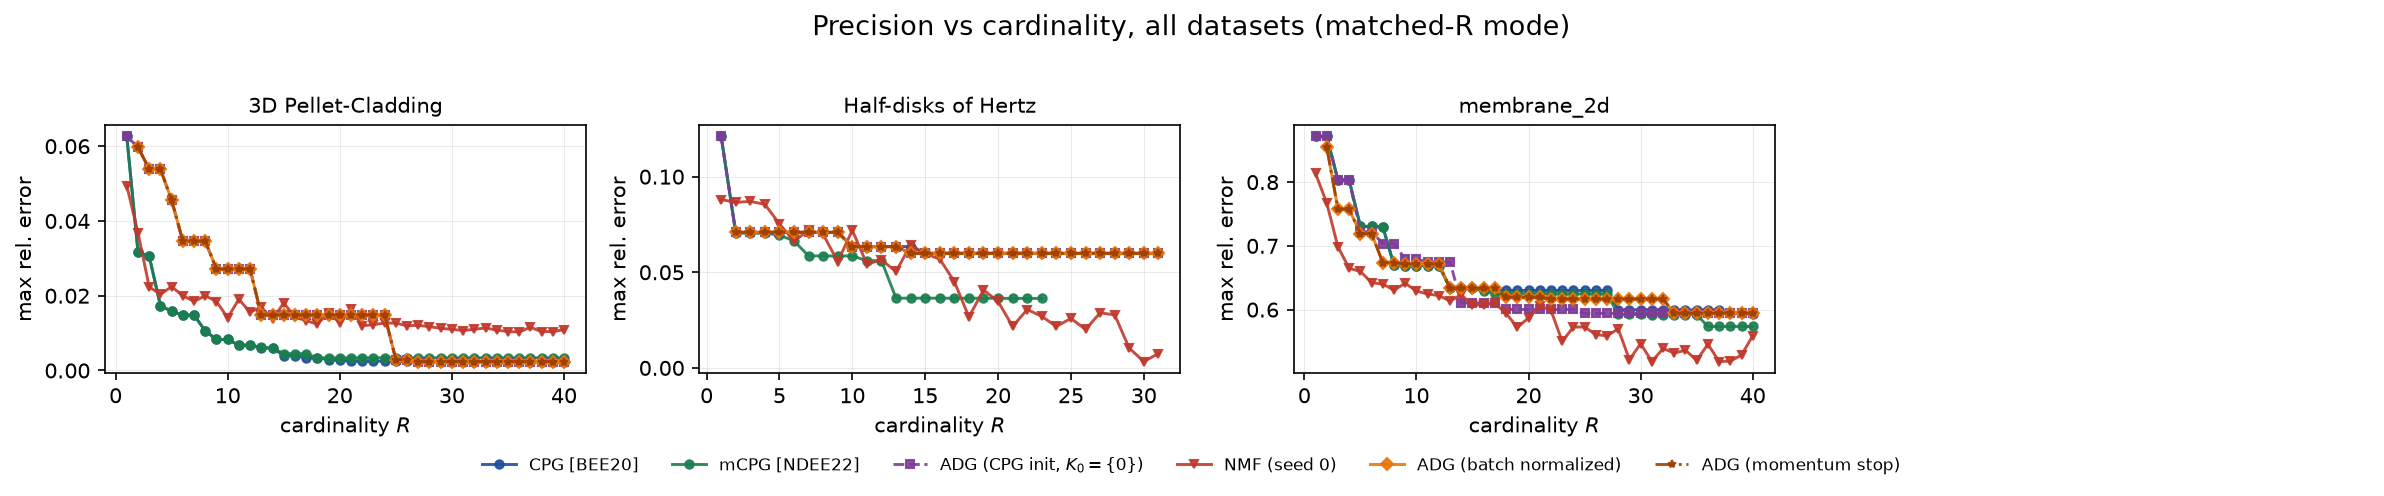
\includegraphics[width=\textwidth]{precision_overview.png}
\caption{Test projection error against cardinality, all three datasets. Compressibility
differs by orders of magnitude: Half-disks and Pellet-Cladding fall steeply, membrane
barely moves --- 125 snapshots on 497 dual dofs with a moving contact patch is simply not
compressible to $R\le40$, which is a property of the problem and not of any method.}
\end{figure}

\subsection{Performance (offline cost)}
Wall-clock is machine-dependent, so the primary cost is a \emph{count of constrained
solver calls} --- NNLS, \texttt{lsq\_linear} and \texttt{minimize} --- captured by
instrumenting the solvers during a fit. One caveat governs its reading: it counts
\emph{constrained} solves only, so NMF records exactly $0$, meaning ``issues none'', not
``is free''. ADG likewise records $0$ at $R=1,2$, because it seeds from a Gram-matrix
argmin and NNLS first appears at $R=3$.

\begin{figure}[htbp]
\centering
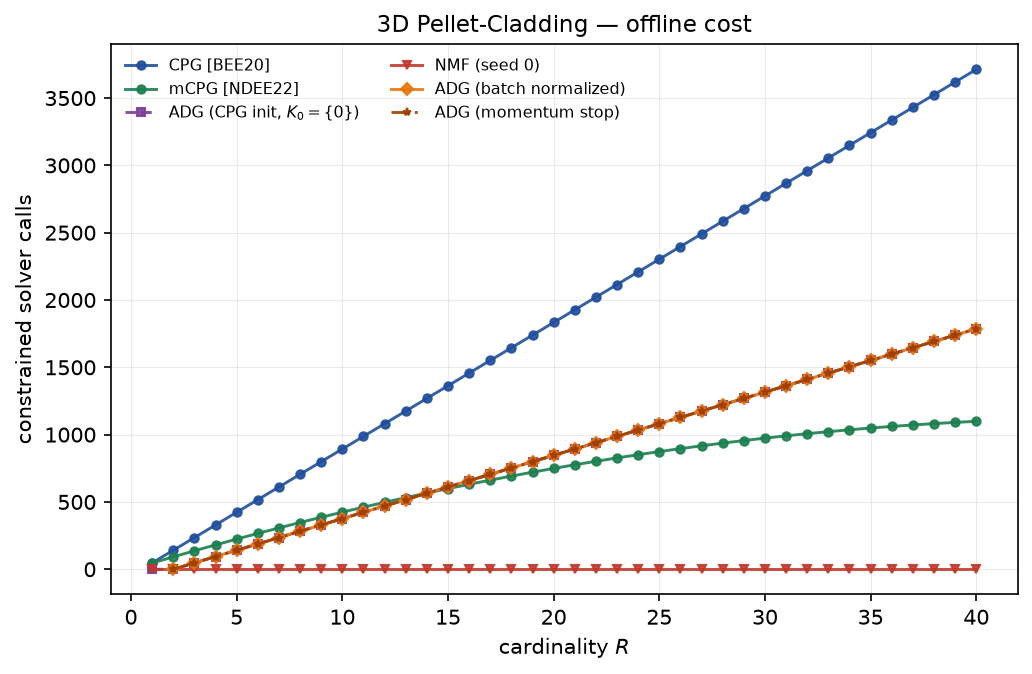
\includegraphics[width=0.72\textwidth]{offline_cost_physics.png}
\caption{Offline cost on 3D Pellet-Cladding. CPG grows about twice as fast as ADG in
constrained solves; mCPG plateaus once its residual stops finding new directions; NMF sits
on the zero line throughout, which means it issues no \emph{constrained} solves, not that
it is free.}
\end{figure}

\subsection{Stability}
\begin{itemize}
\item \textbf{Gram conditioning:} $\kappa(\hat\Xi^{\!\top}\hat\Xi)$ on
\emph{column-normalized} generators. Normalizing is essential: without it the number is
dominated by snapshot magnitude spread, and \bee{} (raw generators) and \ndee{}
(normalized) would be incomparable. Undefined for $R<2$ and reported as such.
\item \textbf{Orthogonality} $e_{\mathrm{orth}}$ (\ndee{}~Eq.~41):
$\|(I-\Pi_{K_r})(\nu_{r+1})\|$, the sine of the angular defect of each accepted generator.
\item \textbf{Determinism:} across-seed spread, which is the non-determinism \bee{}~\S5
raises against NMF.
\end{itemize}

\subsection{Cone geometry}
This family scores the cone against $\Kfull$ rather than against the finite snapshot set,
by Monte-Carlo sampling of Dirichlet$(1)$ conic combinations.
\begin{align}
\text{missed (too small)}&:\quad \mathbb{E}_{x\sim \Kfull}\;\bigl\|x-\Pi_{W_R^+}(x)\bigr\|,\\
\text{excess (too large)}&:\quad \mathbb{E}_{x\sim W_R^+}\;\bigl\|x-\Pi_{\Kfull}(x)\bigr\|,\\
\text{two-sided}&:\quad \tfrac12\bigl(\text{missed}+\text{excess}\bigr).
\end{align}
Neither direction implies the other: a cone can cover $\Kfull$ perfectly while extending
far beyond it, or sit strictly inside while missing most of it. The two-sided figure is
the \emph{average}, not the maximum. A maximum reports only whichever direction is larger
and so silently changes which quantity it plots from one method to the next; the average
is the same functional for every method, keeps both faults in view, and is still a metric
on cones (symmetric, zero only when both vanish, triangle inequality inherited).

\subsubsection*{Extent (how much space the cone encloses)}
Cut $W_R^+$ by a hyperplane $\langle x,u\rangle = h$ shared by every method, with
$u=(1,\dots,1)/\sqrt m$ --- strictly positive on $\Wp\setminus\{0\}$, so the cut is
transversal for every admissible cone, and no coordinate is privileged. The section is the
convex hull of $p_i = h\,\xi_i/\langle \xi_i,u\rangle$, and what is reported is its
\textbf{mean width}, normalized by that of $\Kfull$'s section:
\begin{equation}
\mathrm{extent}(W_R^+) \;=\; \frac{w(S_R)}{w(S_{\mathrm{full}})},
\qquad
w(S) \;=\; \mathbb{E}_{g\sim\mathcal N(0,I_m)}\Bigl[\max_i\langle p_i,g\rangle-\min_i\langle p_i,g\rangle\Bigr].
\end{equation}
Three properties make this the right statistic, and each rules out an alternative that was
tried and discarded:
\begin{itemize}
\item \emph{Measured in the dimension of the space, not the number of generators.} The
$\xi_i$ are $R$ rays in $\R^m$ with $R\ll m$; they are not a basis. Taking the section's
$(R{-}1)$-volume builds the method's cardinality into the yardstick.
\item \emph{Monotone in $R$ by construction.} $W_R^+\subseteq W_{R+1}^+$, so the section
can only grow; more vertices means a maximum over a superset, so the integrand rises
pointwise in $g$. The Gaussian directions are drawn once from a fixed seed, so monotonicity
holds per realization and Monte-Carlo noise cannot manufacture a decrease.
\item \emph{Positive on a thin cone,} where every ambient volume, solid angle or
covered-sphere fraction is identically zero.
\end{itemize}
Values above $1$ are meaningful: the cone is wider than $\Kfull$, which requires leaving
it. Scale-invariance ($\spanp\{c\xi\}=\spanp\{\xi\}$) means generator normalization cannot
affect it.

\begin{figure}[htbp]
\centering
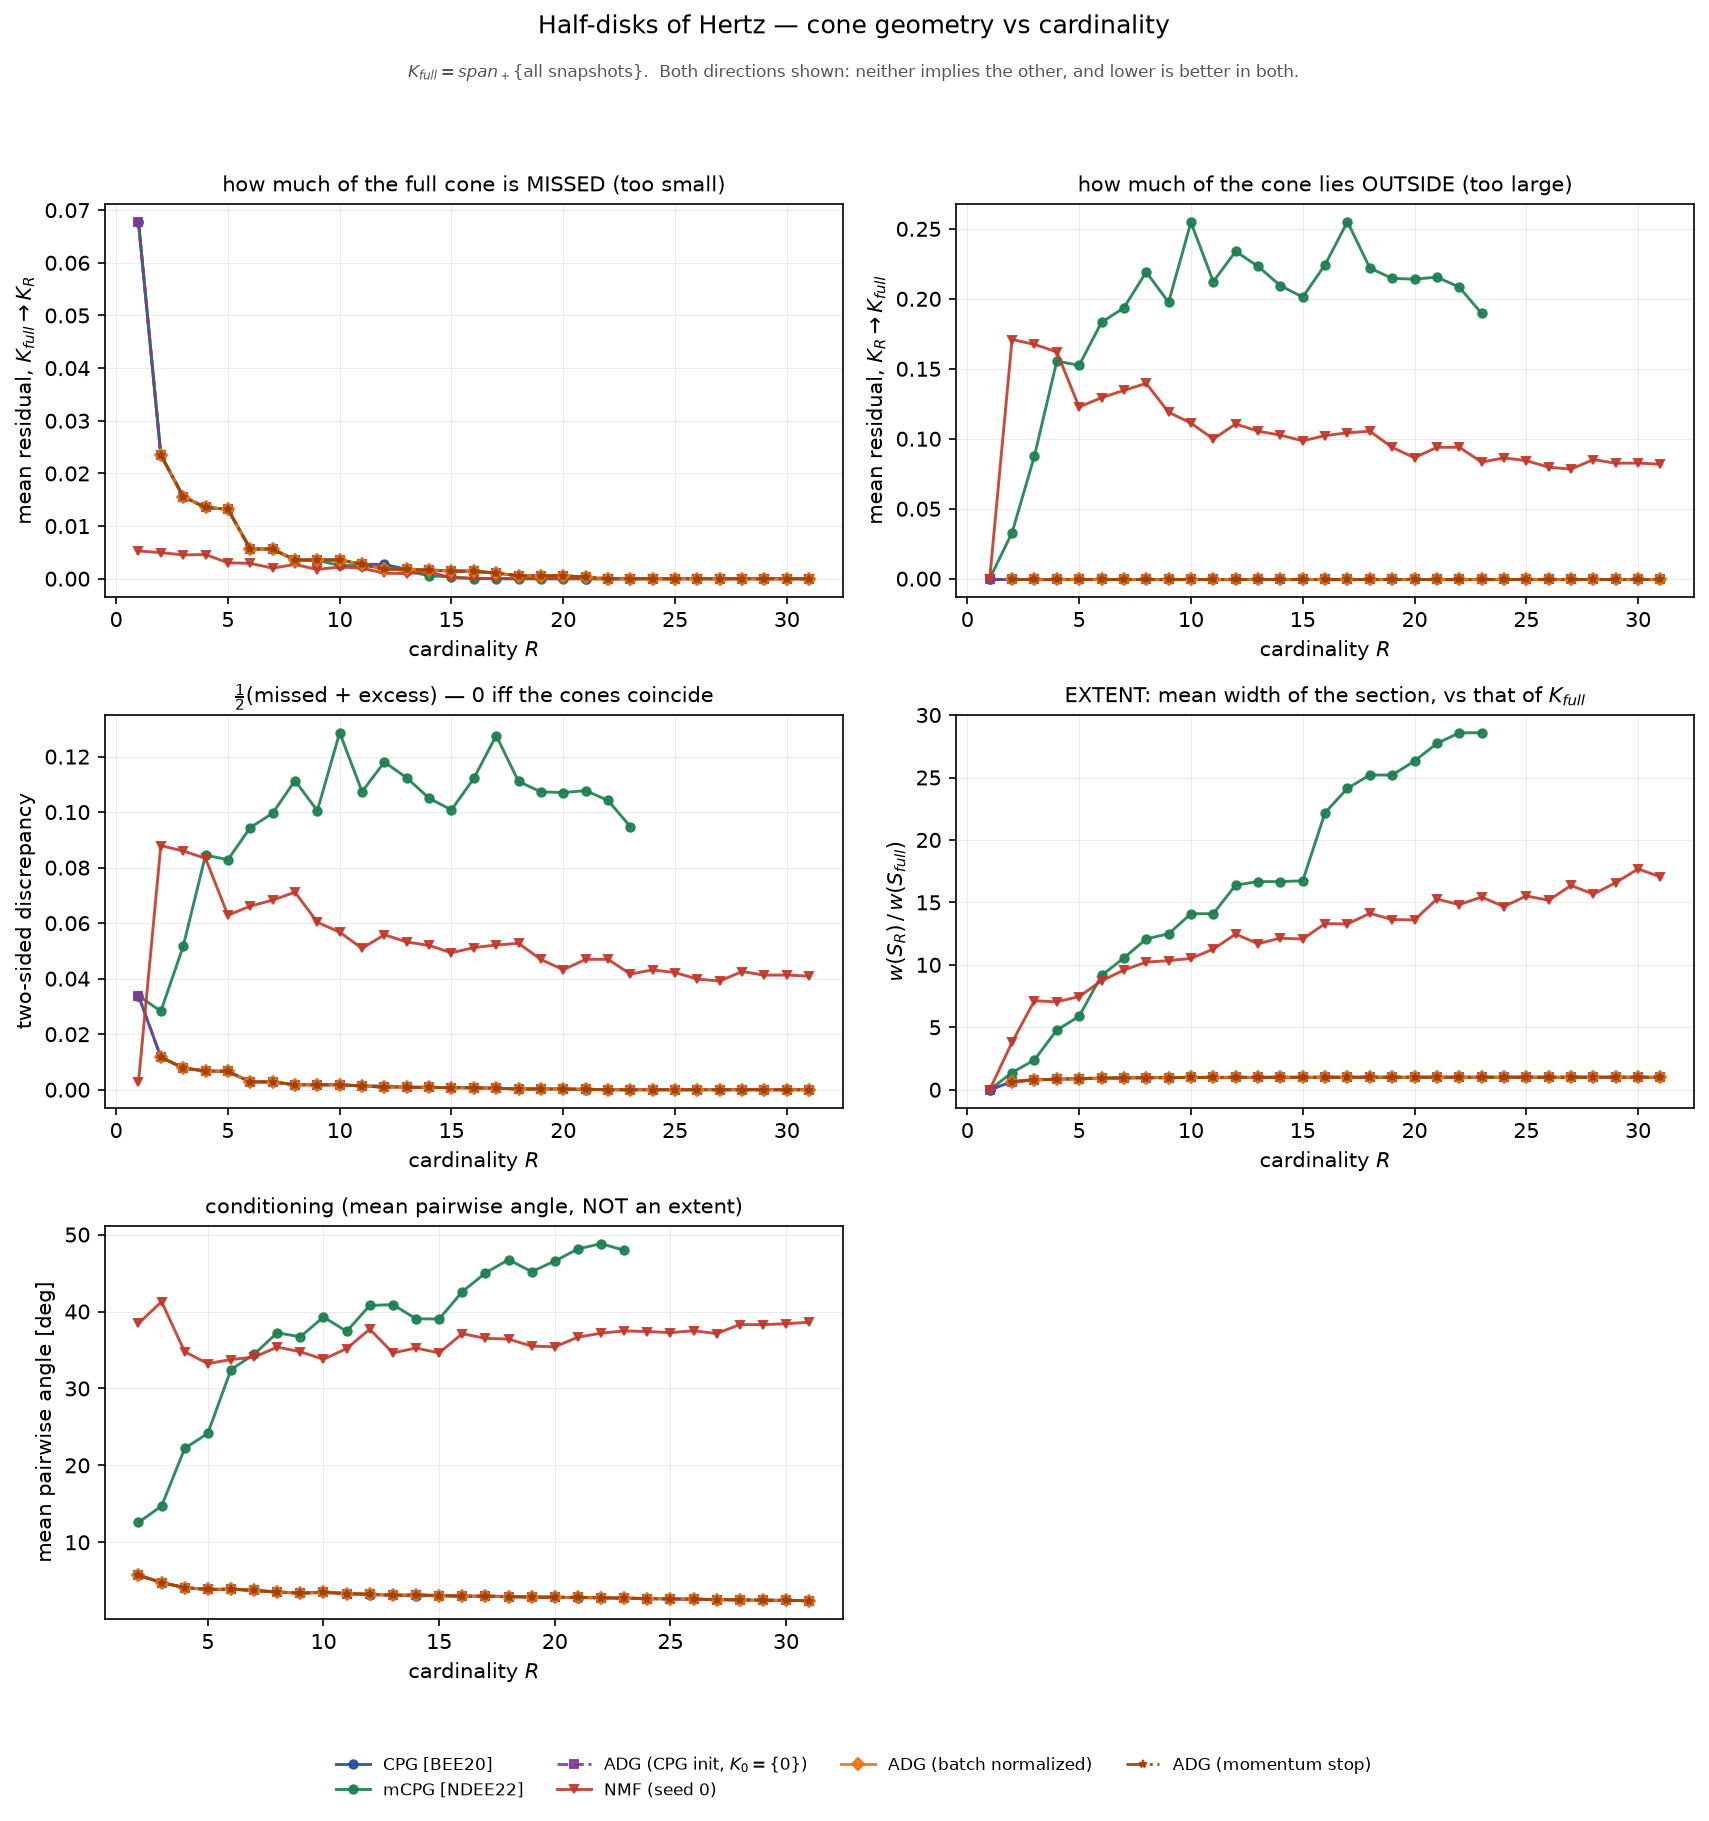
\includegraphics[width=0.92\textwidth]{cone_geometry_halfdisks.png}
\caption{The five cone-geometry panels on Half-disks of Hertz. Read the two residual
panels together: CPG and ADG sit flat at zero in \emph{excess} because a cone spanned by
snapshots cannot leave $\Kfull$, while mCPG lifts to $0.26$. Extent and aperture
disagree by design --- aperture has mCPG rising smoothly while extent shows what the
enclosed region actually does.}
\end{figure}

\subsubsection*{Aperture (conditioning, \emph{not} extent)}
Mean pairwise angle between normalized generators. Retained as a conditioning diagnostic
only. It is not a measure of enclosed space: it saturates once generators are mutually
well separated, and a generator added strictly \emph{inside} the cone enlarges the region
not at all while still moving the mean.

\subsection{Solved error (\texttt{metrics.online})}
Every metric above scores a cone against snapshots; none solves anything. This one
assembles and solves the reduced saddle-point problem (\bee{}~Alg.~1 line 4) at each
held-out parameter,
\begin{equation}
\hat A = V^{\!\top}\!AV,\quad
\hat B = \Xi^{\!\top}\!B(\mu)V,\quad
\min_{\alpha\ge0}\;\tfrac12\alpha^{\!\top}\hat B\hat A^{-1}\hat B^{\!\top}\alpha
- \alpha^{\!\top}\!\bigl(\hat B\hat A^{-1}\hat f-\hat g\bigr),
\end{equation}
and reports the relative error in \emph{both} components against the HF solution. This
is the \emph{dual} form of the reduced problem, obtained by eliminating the primal
coefficients in closed form; it is derived step by step in Appendix~\ref{app:dual}, which
also explains in what sense it is still a projection. The bound $\alpha\ge0$ is the
discrete form of $\spanp$, and it is why the recovered $\hat\lambda=\Xi\alpha$ is
non-negative exactly rather than approximately. Projection
error and solved error are different functionals of the same cone: the solve minimizes an
energy over $W_R^+$, it does not project the true multiplier onto it.

\subsection{Cross-implementation agreement}
Two independent transcriptions of CPG and of mCPG are retained deliberately. Agreement
between them is checked at matched tolerance, so that a disagreement is a \emph{finding}
about an under-specified step rather than a rounding difference.

\section{Experimental protocol}\label{sec:protocol}

\textbf{Datasets.} Three contact problems on real geometry:

\begin{center}
\begin{tabular}{@{}llrl@{}}
\toprule
key & reported name & $\dim\times n$ & geometry \\
\midrule
\texttt{fem\_lambda}  & Half-disks of Hertz  & $57\times 50$   & mirrored contact line \\
\texttt{physics}      & 3D Pellet-Cladding   & $7676\times 94$ & $76\times101$ surface grid \\
\texttt{membrane\_2d} & membrane (2-D)       & $497\times125$  & scattered 2-D patch \\
\bottomrule
\end{tabular}
\end{center}

\textbf{Two modes, never mixed.} \emph{Matched tolerance} gives every method the same
$\varepsilon$ and reports the $R$ it needed; \emph{matched cardinality} gives every method
the same $R$. Only the second is used for comparison figures, because tolerances are not
commensurable across methods (ADG's is per-snapshot relative; CPG/mCPG's is one shared
absolute threshold).

\textbf{One greedy trajectory.} The cardinality sweep re-fits at each $R$. That is only
legitimate if a greedy stopped at $R$ yields exactly the first $R$ generators of a longer
run, so the property is asserted by test rather than assumed --- and testing it found a
real violation, since the upstream fixed-component helper answered $R=1$ for ADG through a
different selection rule.

\textbf{Skips are recorded, never dropped.} A cell that does not run emits a
\texttt{skip\_reason}, because ``not measured here'' and ``scored badly here'' must never
be confusable.

\textbf{Axes.} All figure axes are linear, with one documented exception: the Gram
condition number, which is $\ge1$ by definition (so the zero-dropping failure of a log
axis cannot occur) and spans eleven decades before the basis goes singular.

\section{Results}\label{sec:results}

All numbers below come from the current run (817 of 840 cells; 1848\,s) on the
matched-cardinality sweep $R=1,\dots,40$ over the three datasets. Every comparison is
read off at \textbf{fixed, shared cardinalities} rather than aggregated across $R$ ---
the earlier draft of this report used medians over the whole sweep for several tables,
which blends a method's cheap-$R$ behaviour with its expensive-$R$ behaviour into one
number and can rank two methods in an order neither of their matched-$R$ curves ever
shows. That draft is superseded; every table below states the $R$ it was read at.

\subsection{Non-negativity holds, exactly, for every cone method}
Across all 817 cells and every cone method, the maximum non-negativity violation of the
reconstruction is exactly $0$. This is structural, not numerical: $c\ge0$ and $\xi\ge0$.
The POD negative control behaves as \bee{}~\S5 predicts and fails: at $R=8$ it violates on
$12.9\%$ of entries on Half-disks and $89.4\%$ on Pellet-Cladding. Driven through the
reduced \emph{solve}, POD's recovered multiplier reaches $-195$ where every cone method
returns exactly $0$.

\subsection{Precision and cost at matched cardinality}\label{sec:precost}

The obvious way to summarize a sweep is a median over $R$. It is also the wrong way to
compare methods: the whole point of a reduced basis is \emph{accuracy for a given number
of components}, and a median blends together how a method does at $R=2$ with how it does
at $R=40$, which is not a comparison anyone asked for and can rank two methods in an order
neither of their matched-$R$ curves ever shows. Every number in this section is instead
read off at fixed, shared cardinalities --- $R=4$ (the cheap regime) and $R=16$ (past the
initial transient, and still meaningful on all three datasets, see \S\ref{sec:cond}) ---
directly from the same rows the figures in \S3--4 are drawn from.

\begin{center}
\begin{tabular}{@{}ll rr rr@{}}
\toprule
& & \multicolumn{2}{c}{$R=4$} & \multicolumn{2}{c}{$R=16$} \\
\cmidrule(lr){3-4}\cmidrule(lr){5-6}
dataset & method & test err & solves & test err & solves \\
\midrule
3D Pellet-Cladding & CPG  & \textbf{0.01737} & 329 & \textbf{0.00395} & 1457 \\
                   & mCPG & \textbf{0.01737} & 181 & 0.00451 & 631 \\
                   & ADG  & 0.05388 & \textbf{94}  & 0.01482 & \textbf{658} \\
                   & NMF  & 0.02037 & 0   & 0.01426 & 0 \\
\midrule
Half-disks of Hertz & CPG  & 0.07089 & 217 & 0.05991 & 961 \\
                    & mCPG & \textbf{0.07043} & 117 & \textbf{0.03647} & 375 \\
                    & ADG  & 0.07089 & \textbf{62}  & 0.05991 & \textbf{434} \\
                    & NMF  & 0.08554 & 0   & 0.05692 & 0 \\
\midrule
membrane (2-D) & CPG  & 0.8032 & 700  & 0.6312 & 3100 \\
               & mCPG & 0.8032 & 393  & 0.6286 & 1479 \\
               & ADG  & \textbf{0.7575} & \textbf{200} & 0.6333 & \textbf{1400} \\
               & NMF  & 0.6649 & 0    & \textbf{0.6076} & 0 \\
\bottomrule
\end{tabular}
\end{center}
\noindent Bold marks the lowest error and the fewest \emph{constrained} solves per block;
NMF's $0$ is never bolded as ``cheapest'' since it means ``uncounted'', not ``free''
(\S3.2). Read this against the median table it replaces: on Pellet-Cladding, CPG and mCPG
now visibly \emph{dominate} ADG in error at both cardinalities rather than merely on
average, and NMF is not competitive with any of them there at all --- the opposite
impression a blended number could leave.

\noindent\textbf{The CPG/ADG cost ratio is a function of $R$ alone, not of the dataset.}
Reporting one ``median'' ratio hid that it moves --- and hid the more interesting fact
that, at any fixed $R$, it is \emph{the same number on all three datasets}:

\begin{center}
\begin{tabular}{@{}lrrrr@{}}
\toprule
$R$ & 4 & 8 & 16 & 24 \\
\midrule
solves(CPG)/solves(ADG) & 3.50 & 2.50 & 2.21 & 2.14 \\
\bottomrule
\end{tabular}
\end{center}
\noindent identically, to three significant figures, on 3D Pellet-Cladding, Half-disks and
membrane. Since $\Kfull$'s dimension, geometry and conditioning differ enormously across
the three (Table in \S\ref{sec:cond}), a ratio this exactly reproducible cannot be a
property of the data --- it is combinatorial, fixed by how many constrained solves each
selection rule issues per round ($\S3.2$), and is largest exactly where it matters most:
$3.5\times$ at $R=4$, settling toward $2\times$ by $R\ge24$.

\noindent\textbf{ADG equals CPG exactly on Half-disks, and the reason is measurable.}
The table above shows identical errors for CPG and ADG on Half-disks at both
cardinalities. This is not approximate agreement: their selected snapshot \emph{sets} are
identical at $R=4,8,16,24$, verified directly against \texttt{selected\_indices}. The
cause is that CPG ranks by raw residual magnitude while ADG ranks by angle on normalized
snapshots, and the two rankings coincide whenever snapshot norms are close to uniform ---
which Half-disks' are ($\max/\min=1.09$, $\mathrm{std}/\mathrm{mean}=2.4\%$) and
Pellet-Cladding's emphatically are not ($\max/\min=187$, $\mathrm{std}/\mathrm{mean}=71\%$,
where the two methods select different snapshots and land $3$--$4\times$ apart in error).
Membrane sits between the two ($1.39\times$) and its selections partially agree.

\noindent\textbf{NMF's apparent Half-disks advantage is a rank-cliff artefact, not a
general edge.} At $R=4$ NMF is worse than CPG/ADG (0.0855 vs.\ 0.0709); by $R=16$ it is
narrowly better (0.0569 vs.\ 0.0599). The reason is not that NMF is more accurate --- it
is that CPG and ADG \textbf{freeze}. Their error on Half-disks is exactly $0.0599$ at
every $R=16,17,\dots,31$ (sixteen bit-identical values), because both are confined to the
span of selected snapshots and that span has exhausted the training set's numerical rank
(17 of 31, \S\ref{sec:cliff}) by $R=16$: no further generator can add anything. NMF is
refit from scratch at each $R$ with \emph{optimized} atoms rather than selected snapshots,
so it is not confined to that span and keeps improving past the cliff, reaching $0.0075$
by $R=31$ --- eight times better than CPG/ADG's frozen value. On Pellet-Cladding, which
never hits its rank ceiling in the sweep, no such reversal occurs and CPG/mCPG beat NMF at
every matched $R$ shown.

\subsection{mCPG leaves the snapshot cone, and the fraction grows with $R$}
\ndee{}~Remark 4.3's parenthetical claims $\nu_r$ lies ``in fact of
$\mathrm{Span}^+(\{\theta_{q_n}\})$''. It does not hold as stated, and the extent of the
failure is itself a function of $R$ that a single summary number would flatten:

\begin{center}
\begin{tabular}{@{}lrrrr@{}}
\toprule
dataset & $R=4$ & $R=8$ & $R=16$ & $R=24$ \\
\midrule
3D Pellet-Cladding  & 0.000 & 0.000 & 0.250 & 0.375 \\
Half-disks of Hertz & 0.750 & 0.875 & \textbf{0.938} & --- $^\dagger$ \\
membrane (2-D)      & 0.750 & 0.875 & 0.938 & \textbf{0.958} \\
\bottomrule
\end{tabular}
\end{center}
\noindent$^\dagger$mCPG self-terminates near $R=23$ on Half-disks, so no $R=24$ cell
exists (\S\ref{sec:precost} note on skips). CPG and ADG are $0.000$ at \emph{every}
matched $R$ on all three datasets, as they must be: their generators \emph{are}
snapshots. What \emph{does} hold for mCPG is the $\Wp$ membership the same sentence
claims first, which is the part the construction actually rests on. The extent metric
confirms the escape independently and at the same matched cardinalities: at $R=16$,
mCPG's cone measures $2.80\times$, $22.2\times$ and $0.91\times$ the width of $\Kfull$ on
Pellet-Cladding, Half-disks and membrane respectively --- exceeding $1$ (wider than
everything the snapshots generate) on the two datasets where it is also leaving $\Kfull$
most, which is only possible by construction if it has left.

\subsection{Conditioning at matched cardinality: no method dominates}
Naming one method ``best conditioned'' from an aggregate would repeat the mistake this
section exists to fix. At matched $R$, away from the numerically-singular region
(\S\ref{sec:cond}), the ranking is dataset-specific: ADG leads on Pellet-Cladding at small
$R$ but is overtaken by NMF past $R\approx15$; mCPG is two to four orders of magnitude
better conditioned than CPG/ADG on Half-disks, where the latter two are identical to each
other; and on membrane ADG holds a modest, consistent edge throughout. The full matched-$R$
table is in \S\ref{sec:cond}, which also shows this ranking is not the interesting
regularity --- the \emph{rate} at which conditioning is lost is set by the dataset, far
more than by the method.

\subsection{ADG's pair initialization: mostly irrelevant, and never decisive}
Comparing base ADG against \texttt{adg\_k0} (CPG's first step) at matched $R$:

\begin{center}
\begin{tabular}{@{}lrrr@{}}
\toprule
dataset & pair better & $K_0=\{0\}$ better & identical \\
\midrule
3D Pellet-Cladding  & 0 & 0  & 39 of 39 \\
Half-disks of Hertz & 0 & 0  & 30 of 30 \\
membrane (2-D)      & 12 & \textbf{27} & 0 of 39 \\
\bottomrule
\end{tabular}
\end{center}

\begin{figure}[htbp]
\centering
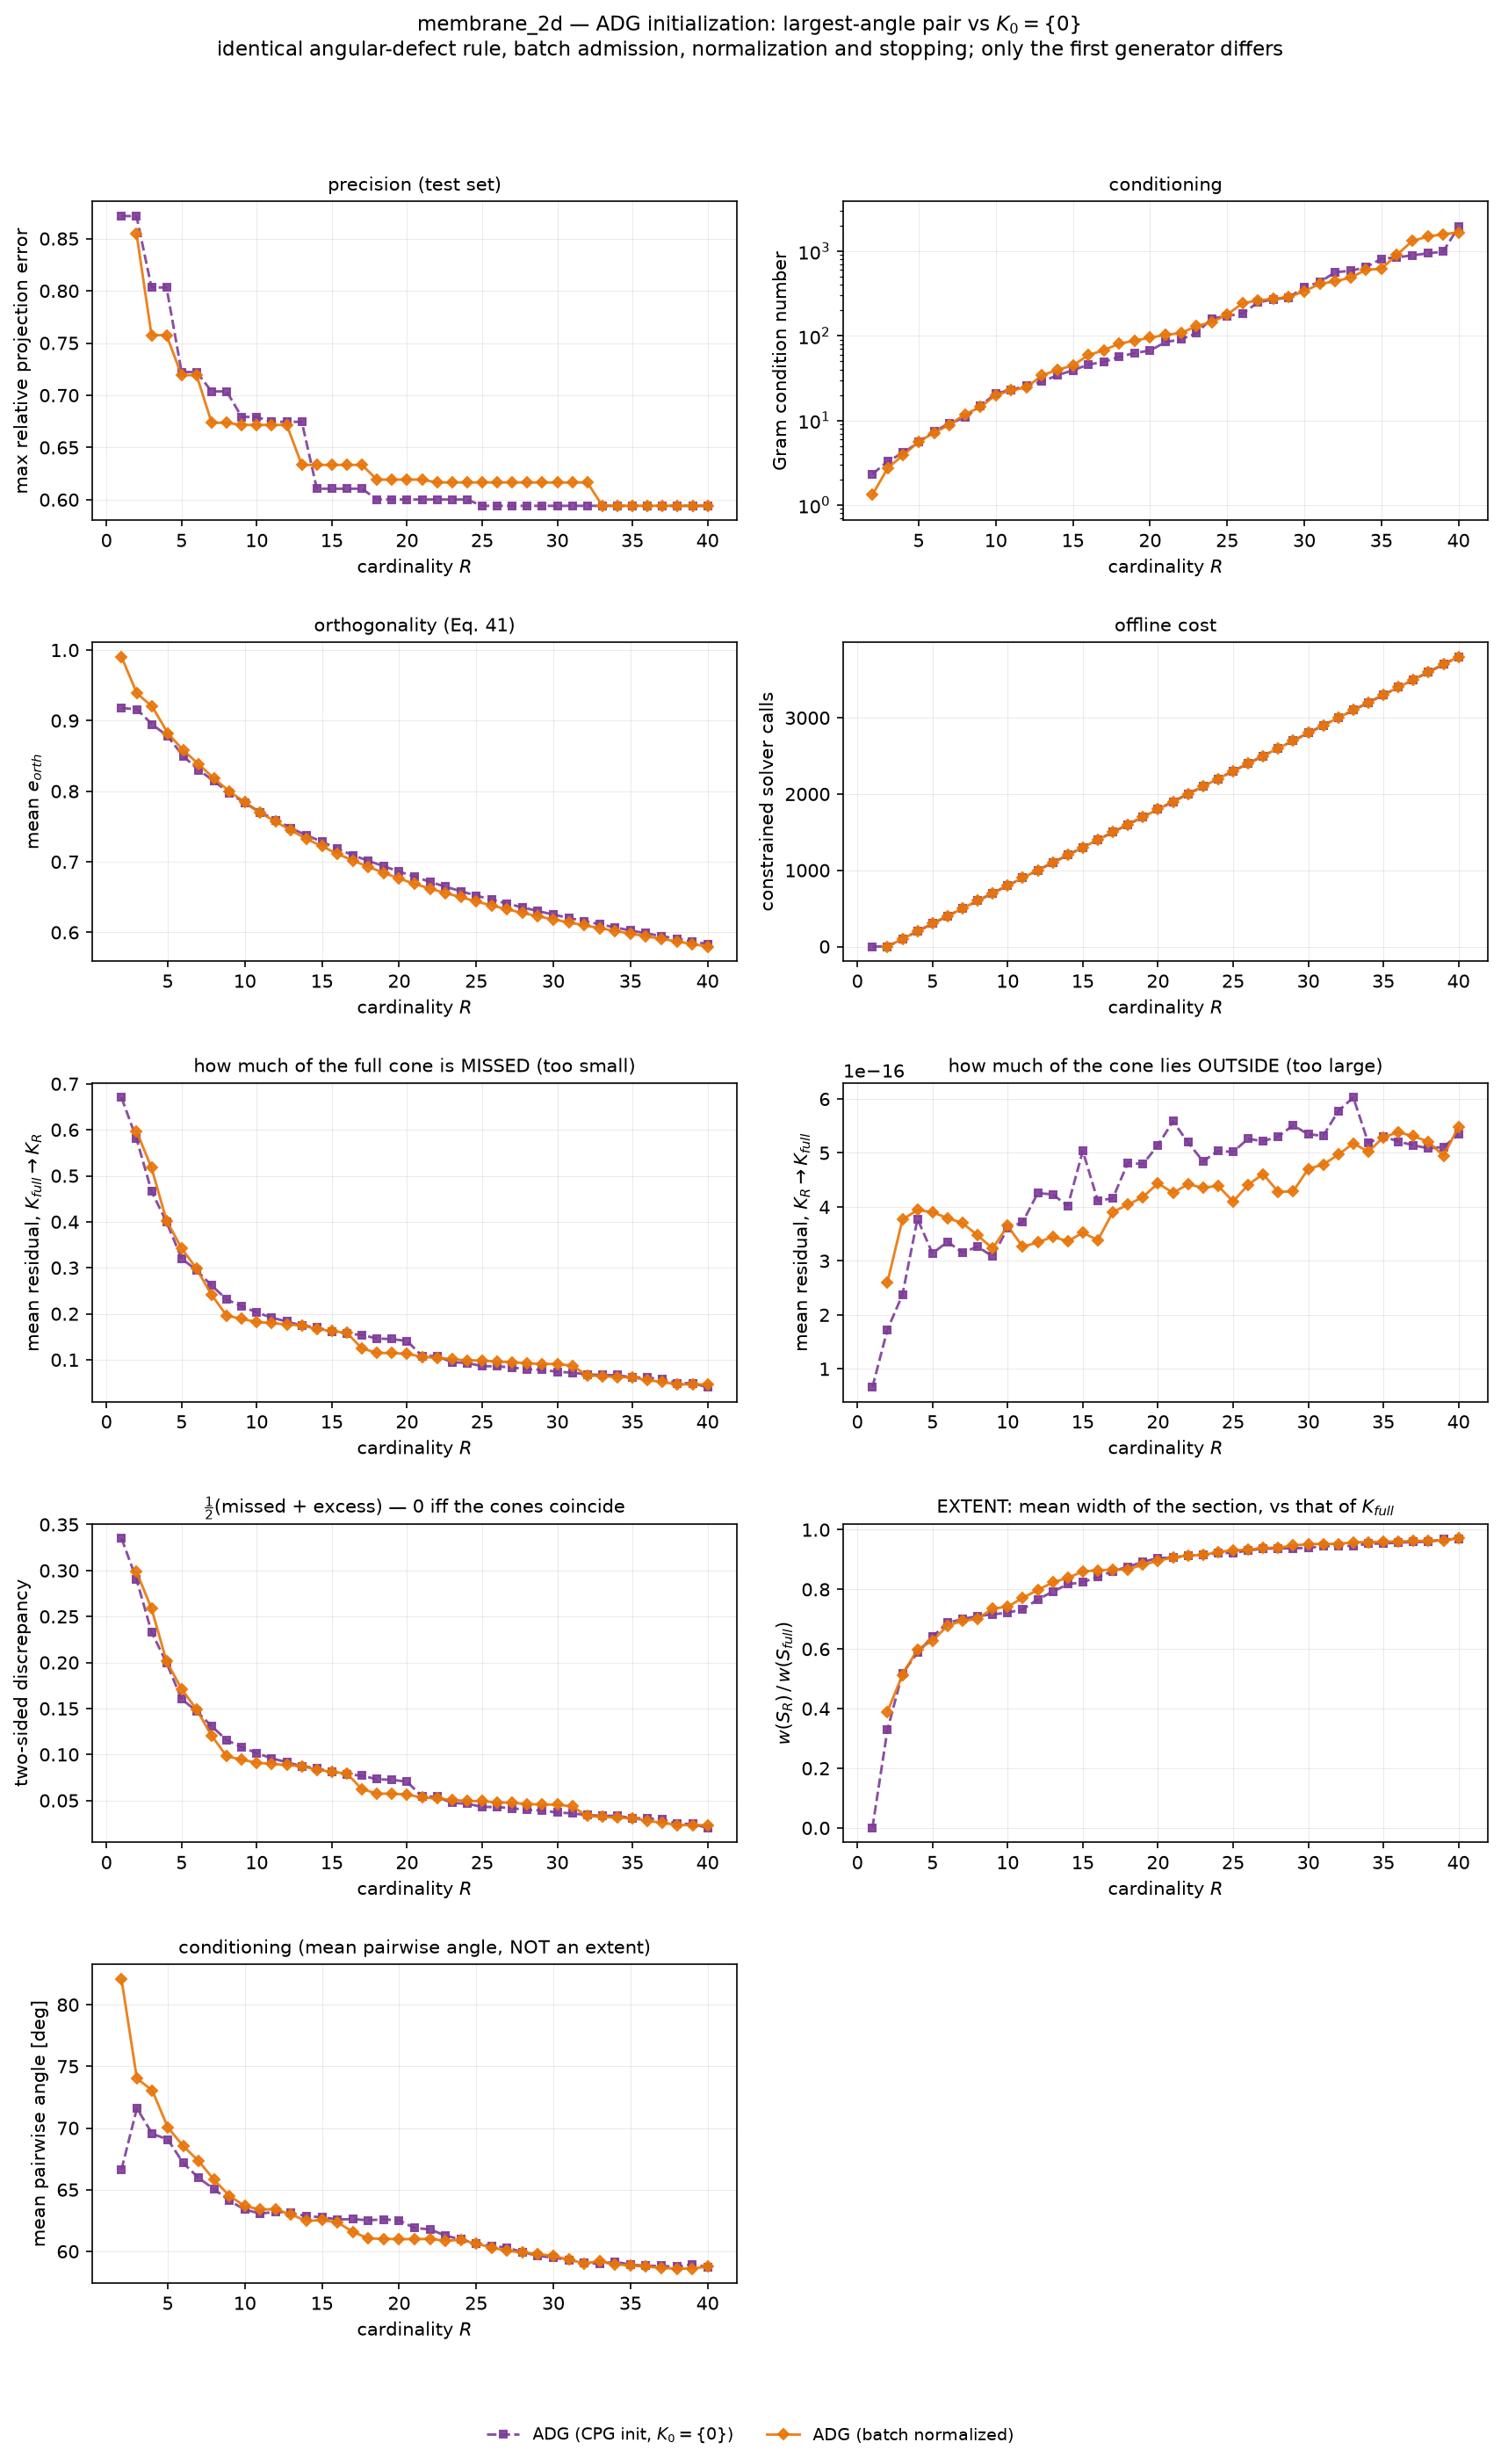
\includegraphics[width=0.88\textwidth]{adg_init_membrane.png}
\caption{The initialization ablation on membrane --- the one dataset of the three where
the two arms differ at all. Every panel is the same algorithm apart from the first
generator. On the other two datasets the curves coincide exactly at every cardinality.}
\end{figure}

\noindent On two of three datasets the two initializations produce \emph{the same cone at
every cardinality}, because the largest-magnitude snapshot already lies in the
largest-angle pair. Where they differ, the CPG-style start wins more often. Offline cost is
unaffected: the choice moves \emph{which} snapshots are selected, never how many solves it
takes. The pair initialization is therefore not earning its departure from the papers on
this evidence.

\subsection{Agreement between the duplicate transcriptions}\label{sec:agree}
CPG's two independent transcriptions agree on \textbf{36 of 36} comparisons. mCPG's do
not: of 18 comparisons, 7 are exactly equivalent, 1 agrees within solver tolerance, 9
produce a \emph{different cone of the same accuracy}, and 1 is genuinely divergent. This
is a finding about \ndee{} Algorithm 2 line 9, whose constrained shift is
under-specified --- the two implementations resolve it with different solvers, and the
resulting cones differ.

\section{Conditioning: a closer study}\label{sec:cond}

Conditioning deserves its own treatment because it is the quantity that decides whether a
cone of a given cardinality is \emph{usable}, independently of how accurate it is. The
reduced solve inverts $\hat A$ and forms $\hat B\hat A^{-1}\hat B^{\!\top}$; recovering
the coefficients $c$ from a cone projection is an NNLS problem on $\Xi$. Both inherit
$\kappa(\hat\Xi^{\!\top}\hat\Xi)$. A cone that reaches a smaller projection error at a
condition number of $10^{17}$ has not necessarily bought anything.

\subsection{What is measured, and on which convention}
$\kappa$ is computed on \textbf{column-normalized} generators, and the choice is not
cosmetic. \bee{}'s CPG keeps raw selected snapshots; \ndee{}'s mCPG normalizes. Measured
on raw generators the number would partly report snapshot magnitude spread rather than
cone geometry, and the two families would not be comparable. Both are recorded; their
ratio shows how much the convention was worth:

\begin{center}
\begin{tabular}{@{}llrrr@{}}
\toprule
dataset & method & $\kappa$ (normalized) & $\kappa$ (raw) & raw/norm \\
\midrule
3D Pellet-Cladding & CPG  & $9.38\times10^{6}$ & $2.42\times10^{6}$ & 0.26 \\
                   & mCPG & $1.12\times10^{7}$ & $1.12\times10^{7}$ & \textbf{1.000} \\
                   & ADG  & $8.15\times10^{4}$ & $1.29\times10^{6}$ & 15.8 \\
\midrule
Half-disks of Hertz & CPG  & $1.38\times10^{17}$ & $5.67\times10^{16}$ & 0.41 \\
                    & mCPG & $1.41\times10^{5}$  & $1.41\times10^{5}$  & \textbf{1.000} \\
\midrule
membrane (2-D) & CPG & $104$ & $96.8$ & 0.93 \\
               & mCPG & $98.1$ & $98.1$ & \textbf{1.000} \\
\bottomrule
\end{tabular}
\end{center}

\noindent mCPG's ratio is exactly $1.000$ on all three datasets, which is the convention
confirming itself: its generators are already unit vectors, so normalizing is the identity
for it. For ADG on Pellet-Cladding the two differ by $15.8\times$ --- had the raw number
been reported, ADG's conditioning advantage there would have been hidden entirely.

\subsection{Conditioning at matched cardinality, before any rate is fitted}

The rate fitted below is a regression over the whole non-singular range, and while it is
a slope rather than a median, it is still a summary that can hide who is ahead \emph{at
any one $R$}. The direct answer to that comes first:

\begin{center}
\begin{tabular}{@{}ll rrrr@{}}
\toprule
dataset & method & $R=5$ & $R=10$ & $R=15$ & $R=20$ \\
\midrule
3D Pellet-Cladding & CPG  & $9.78\!\times\!10^{3}$ & $5.83\!\times\!10^{4}$ & $9.44\!\times\!10^{4}$ & $8.92\!\times\!10^{6}$ \\
                   & mCPG & $9.78\!\times\!10^{3}$ & $5.83\!\times\!10^{4}$ & $8.78\!\times\!10^{4}$ & $6.94\!\times\!10^{6}$ \\
                   & ADG  & $\mathbf{2.19\!\times\!10^{2}}$ & $\mathbf{4.58\!\times\!10^{3}}$ & $3.21\!\times\!10^{4}$ & $7.11\!\times\!10^{4}$ \\
                   & NMF  & $5.44\!\times\!10^{2}$ & $4.28\!\times\!10^{4}$ & $\mathbf{1.61\!\times\!10^{4}}$ & $\mathbf{8.73\!\times\!10^{3}}$ \\
\midrule
Half-disks of Hertz$^\ddagger$ & CPG  & $6.92\!\times\!10^{3}$ & $2.31\!\times\!10^{6}$ & $1.61\!\times\!10^{9}$ & sing. \\
                    & mCPG & $\mathbf{2.99\!\times\!10^{2}}$ & $\mathbf{8.10\!\times\!10^{3}}$ & $\mathbf{5.21\!\times\!10^{6}}$ & sing. \\
                    & ADG  & $6.92\!\times\!10^{3}$ & $2.31\!\times\!10^{6}$ & $1.61\!\times\!10^{9}$ & sing. \\
                    & NMF  & $7.64\!\times\!10^{3}$ & $5.24\!\times\!10^{4}$ & $7.98\!\times\!10^{5}$ & sing. \\
\midrule
membrane (2-D) & CPG  & $5.99$ & $25.1$ & $52.8$ & $98.1$ \\
               & mCPG & $5.99$ & $25.1$ & $50.0$ & $91.8$ \\
               & ADG  & $\mathbf{5.61}$ & $\mathbf{20.0}$ & $\mathbf{44.6}$ & $\mathbf{95.1}$ \\
               & NMF  & $9.24$ & $14.1$ & $15.7$ & $15.0$ \\
\bottomrule
\end{tabular}
\end{center}
\noindent$^\ddagger$$R=20$ on Half-disks is past the numerical-rank cliff at $R\approx17$
(\S\ref{sec:cliff}); the basis is numerically singular there and any ranking would be
comparing round-off, so the column is intentionally left blank rather than filled with
noise. Bold marks the best-conditioned method in each cell.

\noindent No method wins everywhere, and the earlier report's claim that ADG is simply
``the best conditioned of the greedy methods'' does not survive contact with this table:
it is correct on membrane and at small $R$ on Pellet-Cladding, but \textbf{mCPG is two to
four orders of magnitude better conditioned than CPG and ADG on Half-disks} ($299$ against
$6923$ at $R=5$; $8.1\times10^{3}$ against $2.3\times10^{6}$ at $R=10$), and \textbf{NMF
overtakes ADG on Pellet-Cladding} once $R\gtrsim15$. CPG and ADG are identical on
Half-disks for the reason given in \S\ref{sec:precost} --- coincident selection under a
near-uniform snapshot spectrum --- so the mCPG gap there is not ``mCPG beats CPG and ADG''
so much as ``mCPG picks a different, and much better conditioned, cone.''

\subsection{Growth is geometric in $R$, at a rate set by the dataset}

\begin{figure}[htbp]
\centering
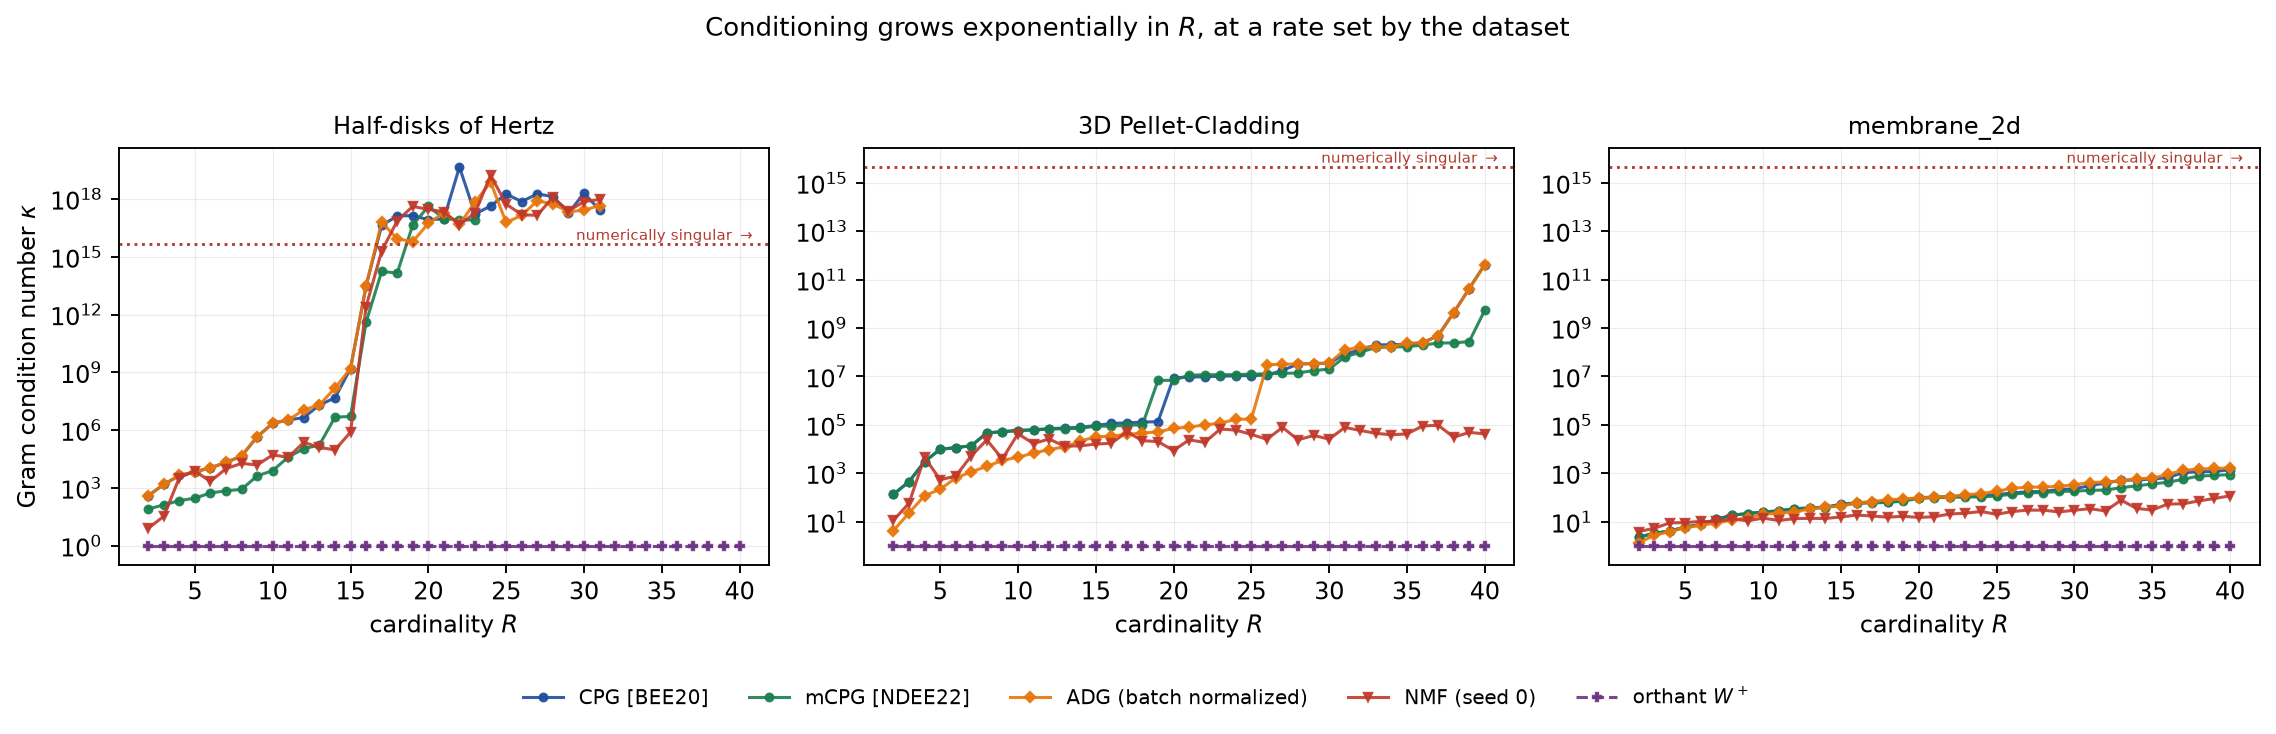
\includegraphics[width=\textwidth]{conditioning_growth.png}
\caption{$\kappa$ against cardinality. Note the log axis --- this is the one panel in the
benchmark that uses one, because $\kappa\ge1$ by definition so the zero-dropping failure
of a log scale cannot occur, and the quantity spans eleven decades. The orthant sits at
exactly $1$ at every $R$: its generators are mutually orthogonal, so it is the
best-conditioned admissible cone there is, and it bounds every curve from below.}
\end{figure}

\noindent Beyond who is ahead at a given $R$, the matched-$R$ table above already shows a
second, orthogonal question: how fast does each curve \emph{move}. On a log axis the
curves are close to straight over most of their range, i.e.\ $\kappa$ grows geometrically
with each added generator --- with one important exception, Half-disks, taken up in
\S\ref{sec:cliff}. Fitting $\log_{10}\kappa$ against $R$ over the non-singular range gives
the rate in \emph{decades gained per generator}:

\begin{center}
\begin{tabular}{@{}lrrrr@{}}
\toprule
dataset & CPG & mCPG & ADG & NMF \\
\midrule
3D Pellet-Cladding  & 0.180 & 0.157 & 0.222 & \textbf{0.051} \\
Half-disks of Hertz & 0.572 & 0.705 & 0.586 & 0.608 \\
membrane (2-D)      & 0.063 & 0.057 & 0.071 & \textbf{0.027} \\
\bottomrule
\end{tabular}
\end{center}

\noindent The rate is a property of the \emph{dataset} far more than of the method: it
varies by a factor of ten across datasets and by well under two across methods on any one
of them. NMF is consistently the gentlest, which is what one expects from atoms that are
optimized rather than selected --- it is free to place a generator where it improves
conditioning, whereas a greedy must take a snapshot that exists.

\subsection{The collapse is the snapshot spectrum, not the algorithm}\label{sec:cliff}

The Half-disks rates above are misleading taken alone, and the figure shows why: that
dataset does not decay geometrically at all. It is flat to $R\approx15$ and then falls off
a cliff, with every method collapsing together within two cardinalities of each other
($R=17$ for CPG and ADG, $18$ for NMF, $19$ for mCPG). A single fitted slope averages
across that cliff and describes neither side of it.

\begin{figure}[htbp]
\centering
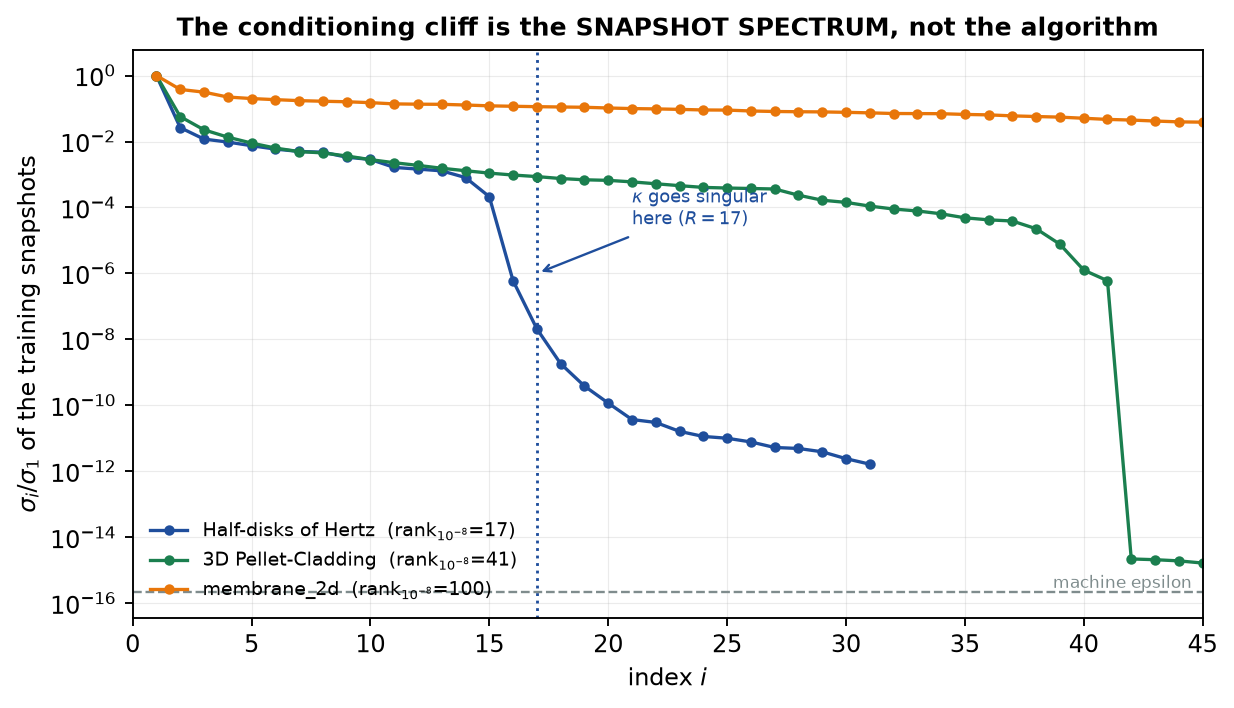
\includegraphics[width=0.78\textwidth]{spectra.png}
\caption{Normalized singular values of the training snapshots. The Half-disks spectrum
drops from $\sigma_{14}=2.1\times10^{-4}$ to $\sigma_{15}=6.0\times10^{-7}$ to
$\sigma_{16}=2.1\times10^{-8}$ --- three decades in two indices. That cliff is at exactly
the cardinality where every method's conditioning explodes.}
\end{figure}

\noindent The explanation is the numerical rank of the snapshot set:

\begin{center}
\begin{tabular}{@{}lrrrl@{}}
\toprule
dataset & $\dim\times n_{\mathrm{train}}$ & $\sigma_2/\sigma_1$ & rank$_{10^{-8}}$ & conditioning behaviour \\
\midrule
Half-disks of Hertz & $57\times31$   & 0.026 & 17 of 31  & flat, then a cliff at $R\!\approx\!16$ \\
3D Pellet-Cladding  & $7676\times47$ & 0.057 & 41 of 47  & smooth staircase, never singular \\
membrane (2-D)      & $497\times100$ & 0.380 & 100 of 100 & gentle, $\kappa<10^{4}$ throughout \\
\bottomrule
\end{tabular}
\end{center}

\noindent Once $R$ exceeds the numerical rank, any further generator is a numerically
dependent combination of those already selected, and no selection rule can avoid it: the
information is not in the data. This is the single most useful conditioning result in the
benchmark, because it is \emph{predictive} --- the spectrum is computable before any
method runs, and it says where the usable range ends. On Half-disks that is
$R\approx15$, and reporting a Half-disks result at $R=30$ is reporting round-off.

\subsection{Conditioning against ADG's own stopping criterion}\label{sec:theta-kappa}

\S\ref{sec:cliff} located the cliff in $R$, which requires already knowing the numerical
rank in advance. ADG does not need that: at every round it computes
$\theta_{\max}=\max_{q\ \mathrm{unresolved}}\theta_{K}(x_q)$, the worst remaining angular
defect, and compares $\sin\theta_{\max}$ against its tolerance to decide whether to keep
going (\S2.3). This is the quantity the algorithm itself watches as it iterates, so the
three figures below follow ADG's own trajectory on each dataset: every marker is one
round of \texttt{compute\_phases()}, placed at the $\theta_{\max}$ ADG reported for that
round and at $\kappa$ read from the matching cardinality in the same matched-cardinality
grid as every other figure in this report (so $\kappa$ is not recomputed, only relocated
onto this axis). A handful of markers are labelled with the cardinality $R$ they
correspond to, so the two axes used elsewhere --- iteration count and angular error ---
can be read off the same curve.

\begin{figure}[htbp]
\centering
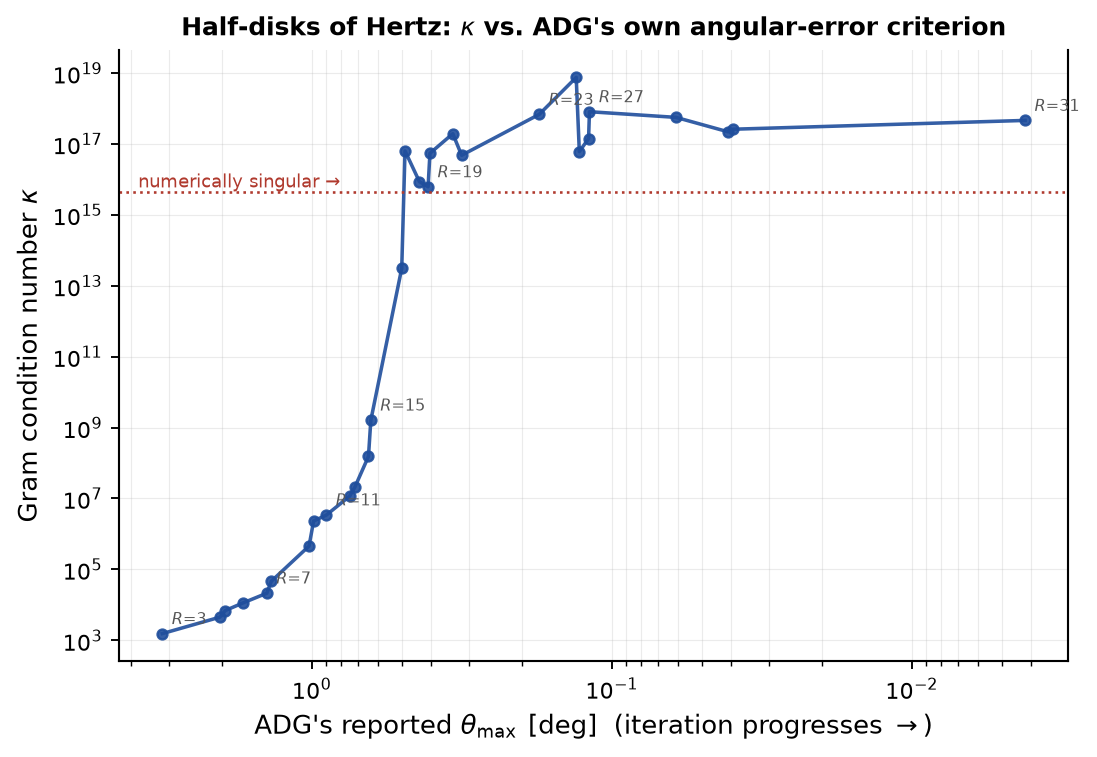
\includegraphics[width=0.74\textwidth]{theta_kappa_halfdisks.png}
\caption{Half-disks of Hertz. $\kappa$ is flat and modest ($10^{3}$--$10^{6}$) for every
$\theta_{\max}\gtrsim2^{\circ}$ (through $R=15$), then rises twelve orders of magnitude
while $\theta_{\max}$ moves from about $2^{\circ}$ to $0.5^{\circ}$ (R=16 to 19) --- under
a factor of four in the criterion itself triggers the entire collapse. Points past the
singular line ($R\ge17$) wobble rather than climb monotonically, confirming they are
round-off on an already-singular Gram matrix (\S\ref{sec:cliff}), not a second effect the
criterion is tracking.}
\end{figure}

\begin{figure}[htbp]
\centering
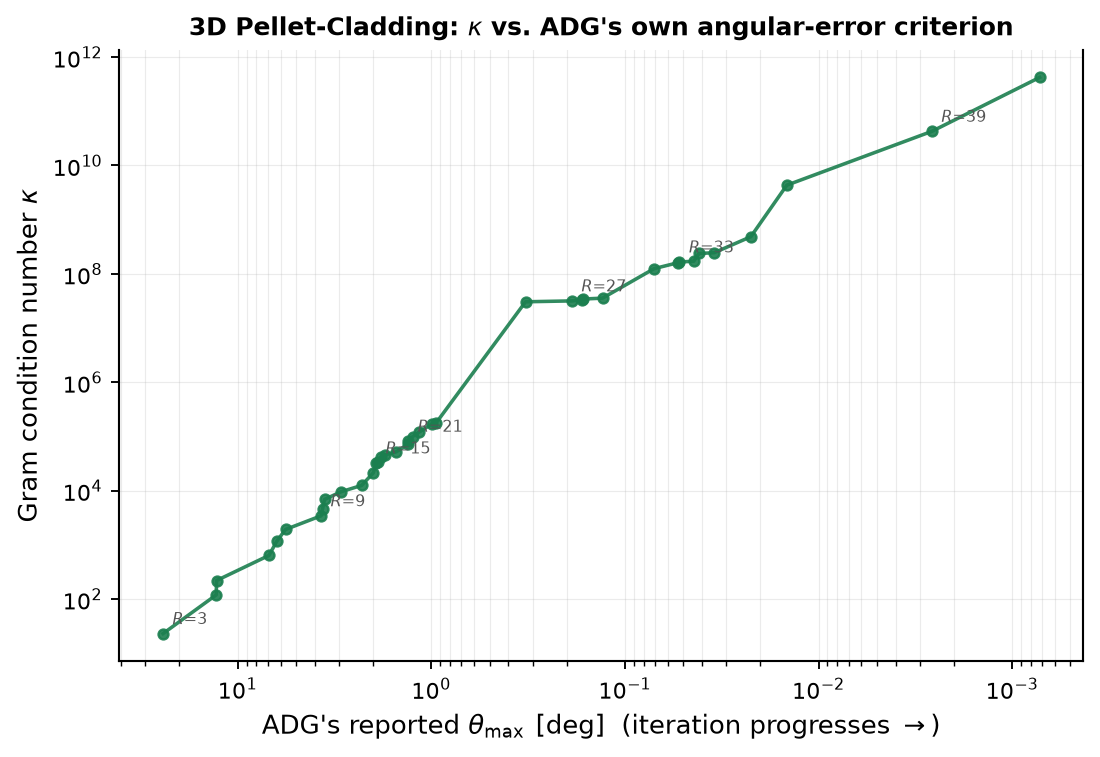
\includegraphics[width=0.74\textwidth]{theta_kappa_pellet.png}
\caption{3D Pellet-Cladding. The curve is smooth and monotonic across nearly five decades
of $\theta_{\max}$ (from $24^{\circ}$ at $R=3$ down to $7\times10^{-4\circ}$ at $R=40$)
with no cliff and no crossing of the singular threshold anywhere in the sweep ---
consistent with its numerical rank (41 of 47) never being exhausted at $R\le40$. Every
added generator buys a roughly constant fraction of the remaining angular error, which is
exactly the geometric decay \S\ref{sec:cliff}'s table already reported from the $\sigma_i$
spectrum, now shown as ADG experiences it round by round.}
\end{figure}

\begin{figure}[htbp]
\centering
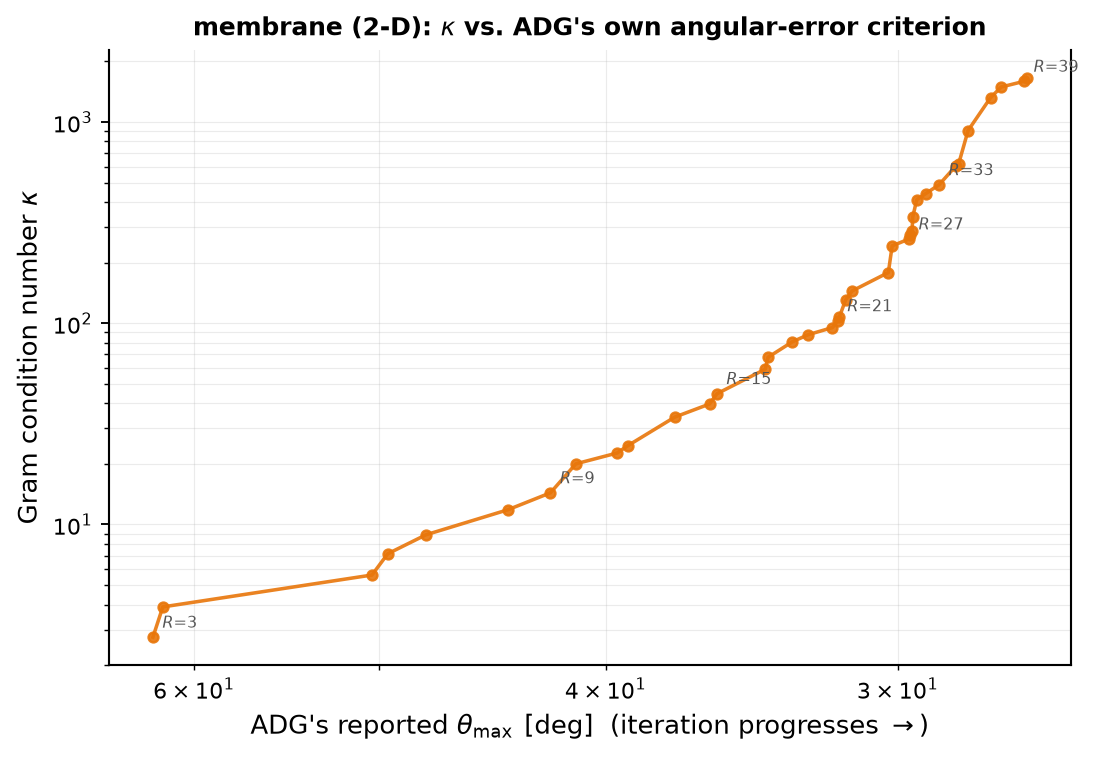
\includegraphics[width=0.74\textwidth]{theta_kappa_membrane.png}
\caption{Membrane (2-D). Within $R\le40$, $\theta_{\max}$ has fallen only from
$62^{\circ}$ (R=3) to $26^{\circ}$ (R=39) --- axis note: $\theta_{\max}$ still decreases
left to right as in the other two panels, but the whole panel occupies the \emph{loose}
end of the range those cover. By ADG's own criterion the greedy has barely begun to
converge, the same conclusion \S\ref{sec:precost} reached from the error curve (membrane
is simply not compressible to $R\le40$), now visible directly in the algorithm's internal
state rather than inferred from its output. $\kappa$ stays three orders of magnitude below
the singular threshold throughout, so this dataset's difficulty is compressibility, not
conditioning.}
\end{figure}

\noindent The practical reading, common to all three: on Half-disks and Pellet-Cladding,
$\theta_{\max}$ dropping below roughly one degree is where conditioning risk stops being
hypothetical, regardless of what $R$ that happens to correspond to on a given dataset ---
membrane never gets there within $R\le40$, which is itself the finding for that dataset.
Because $\theta_{\max}$ is computed anyway, on every round, watching it costs nothing
extra and needs no advance knowledge of the snapshot spectrum --- unlike the rank
criterion in \S\ref{sec:cliff}, which has to be computed once up front and does not
update as the greedy proceeds.

\subsection{Conditioning and aperture measure the same thing from two sides}

\begin{figure}[htbp]
\centering
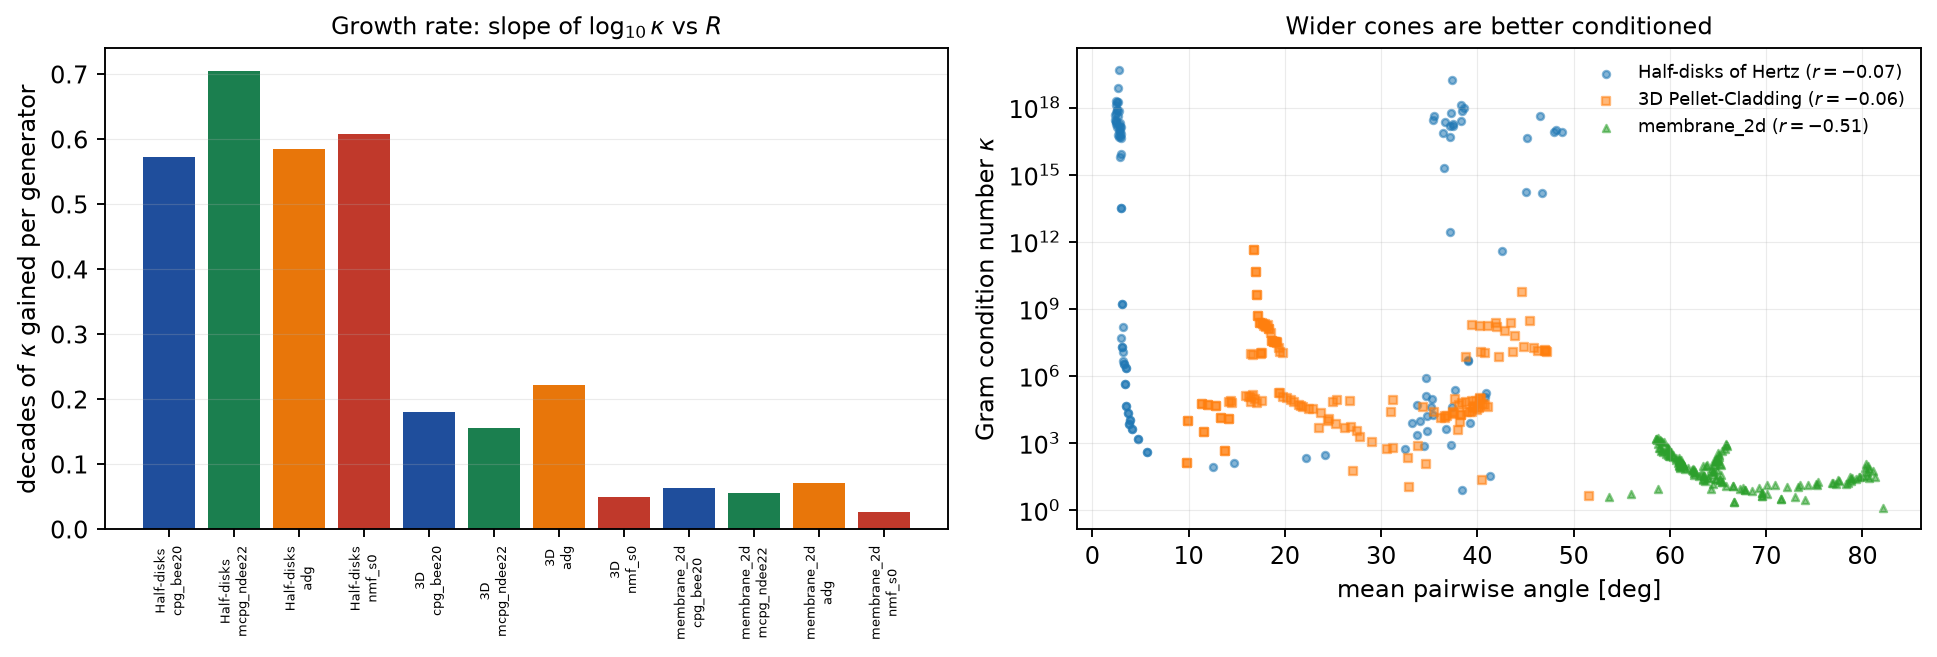
\includegraphics[width=\textwidth]{conditioning_rate.png}
\caption{Left: growth rate per method and dataset. Right: $\kappa$ against mean pairwise
angle, pooled over methods and cardinalities.}
\end{figure}

\noindent The correlation between $\log_{10}\kappa$ and mean pairwise angle is
$-0.70$, $-0.59$ and $-0.81$ on the three datasets: wider cones are better conditioned,
consistently and strongly. This is why aperture is retained as a \emph{conditioning}
diagnostic in \S3.4 and explicitly not as a measure of extent --- it tracks $\kappa$,
which is what \ndee{}~\S4 is after when it asks for a well-conditioned Gram matrix, and it
does \emph{not} track how much space the cone encloses.

\subsection{Which method to prefer, on conditioning grounds}
There is no single answer, and the matched-$R$ table in
\S\ref{sec:precost} and \S\ref{sec:cond} are what replace the single answer an earlier version
of this report gave. Three genuinely different regimes hold:

\begin{itemize}
\item \textbf{Pellet-Cladding.} ADG is markedly better conditioned than CPG/mCPG at small
$R$ --- $\kappa=2.2\times10^{2}$ against $9.8\times10^{3}$ at $R=5$, a factor of $45$ ---
consistent with its selection rule: choosing by \emph{angular} defect rather than residual
magnitude is, almost by definition, choosing generators far from the span already held.
That advantage over CPG/mCPG persists to $R=20$ ($7.1\times10^{4}$ against
$8.9\times10^{6}$, a factor of $125$), but \emph{NMF} overtakes ADG itself by
$R\approx15$, so ``ADG is best'' is only true if the comparison set excludes the baseline.
\item \textbf{Half-disks.} Below the rank cliff, mCPG is dramatically ahead of both CPG
and ADG (two to four orders of magnitude, above), which are identical to each other and
to no one's advantage. Past the cliff every method is numerically singular and no
ranking is meaningful.
\item \textbf{Membrane.} ADG holds a modest, consistent edge over CPG and mCPG throughout
(10--30\%), while NMF is decisively best-conditioned of all four ($15$--$16$ against
$\kappa\gtrsim90$ for every cone method by $R=20$) --- unsurprising, since it is not
confined to selecting from a snapshot set at all.
\end{itemize}

\noindent The one claim that \emph{does} generalize is the one in \S\ref{sec:cliff}: the
numerical rank of the training snapshots bounds every method identically and is
computable before any of them runs, which is more actionable than knowing which greedy
algorithm has a conditioning edge within that bound.

\section{The $\gamma$ family: what the weighting buys}\label{sec:gamma}

\S\ref{sec:gammadef} defines the interpolation \eqref{eq:gamma} between CPG's absolute
criterion ($\gamma=0$) and the normalized one ($\gamma=1$), and establishes that both
endpoints are reproduced exactly and that the offline cost is independent of $\gamma$.
What remains is empirical: whether the intermediate members are worth using. The sweep is
$\gamma\in\{0,0.25,0.5,0.75,1\}$ at $R=1,\dots,40$ on all three datasets.

\begin{figure}[htbp]
\centering
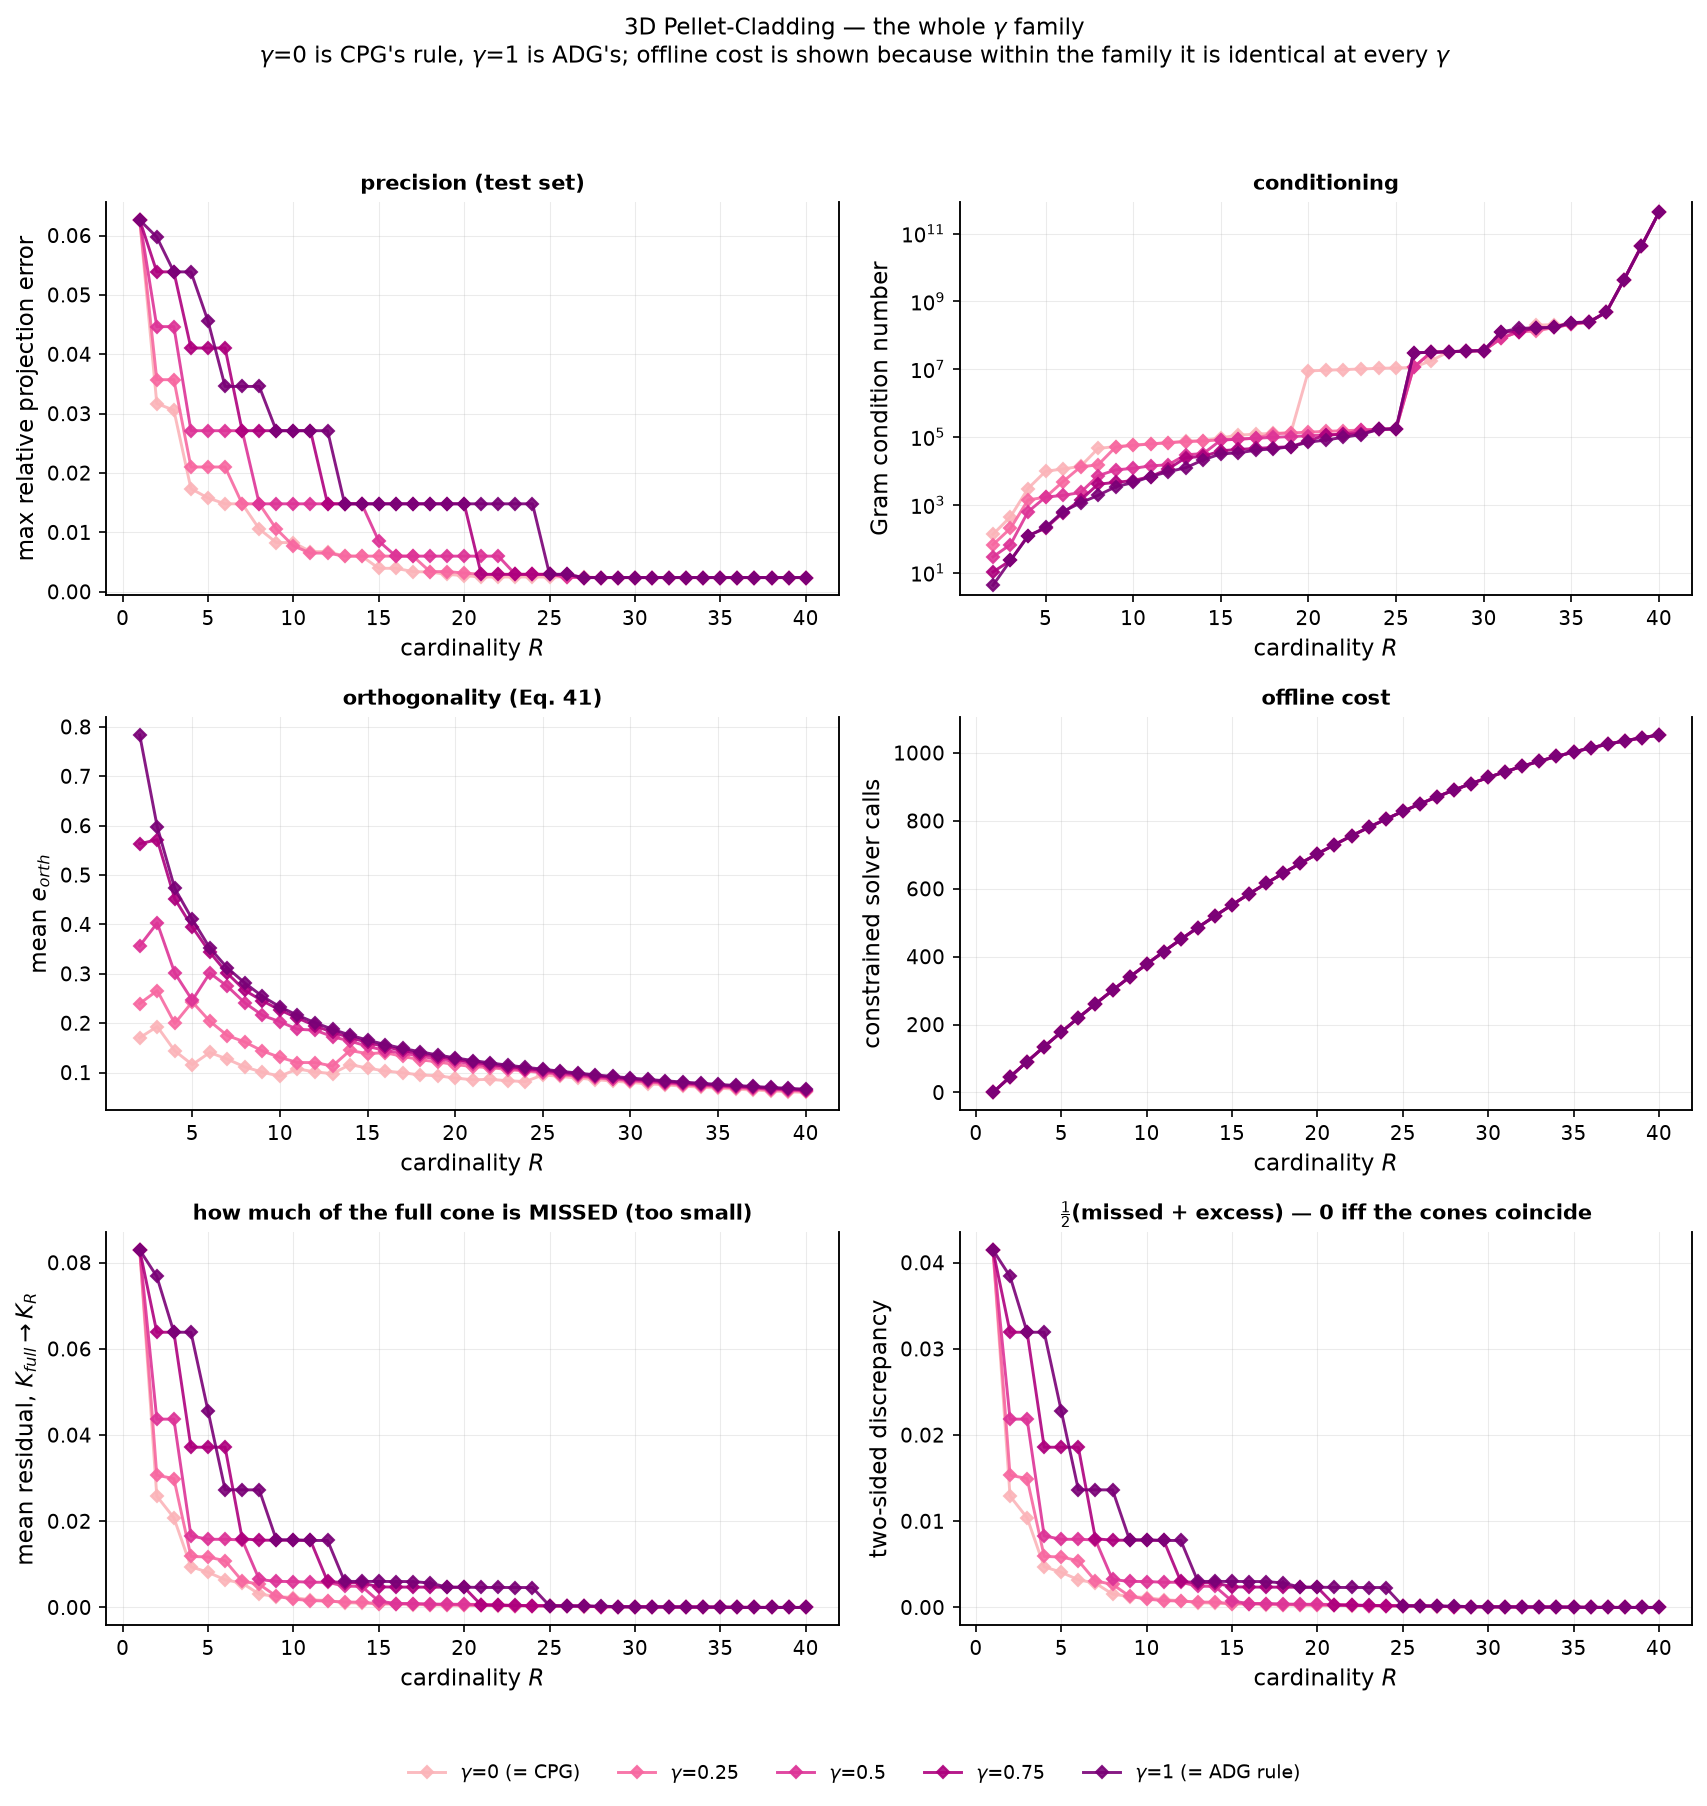
\includegraphics[width=\textwidth]{gamma_family_pellet.png}
\caption{The whole family on 3D Pellet-Cladding. Precision and the two cone-residual
panels show a clean monotone fan in $\gamma$: every member reaches the same floor, higher
$\gamma$ simply reaches it later ($R\approx15$ at $\gamma=0$ against $R\approx25$ at
$\gamma=1$), so the cost of the weight is a \emph{delay} rather than a worse asymptote.
The offline-cost panel has all five curves exactly superimposed --- this is the panel that
shows the knob is free. Conditioning is the one panel where the ordering is not monotone
throughout: it inverts near $R\approx20$, discussed below.}
\label{fig:gammafamily}
\end{figure}

\subsection{Only one dataset can respond to $\gamma$, and it is predictable in advance}

The norm spread $\sigma=\max_q\|\theta_q\|/\min_q\|\theta_q\|$ is $1.086$ on Half-disks,
$1.386$ on membrane and $186.85$ on Pellet-Cladding, and it bounds how far reweighting can
move the selection. The prediction that only Pellet-Cladding can respond is confirmed, and
on Half-disks it is confirmed in the strongest form: \textbf{below the numerical rank
cliff ($R<17$, \S\ref{sec:cliff}) the four nonzero $\gamma$ give error and $\kappa$
identical to CPG's at 13 of 15 cardinalities}, to every printed digit. The two exceptions
are $R=12$ and $R=14$, where $\gamma\ge0.75$ selects differently: at $R=14$ it is $5.6\%$
\emph{more} accurate ($0.0599$ against $0.0634$) and $3.2\times$ worse conditioned
($1.54\times10^{8}$ against $4.79\times10^{7}$).

This deserves emphasis because the aggregate statistics say something different and are
misleading. Over the full $R=2\ldots31$ range the $\gamma$ members show a 90th-percentile
conditioning gain of $\approx18\times$ and a maximum near $10^{3}\times$ on Half-disks.
Every one of those gains falls at $R\ge17$, where the Gram matrix is numerically singular
and $\kappa$ is round-off rather than a measurement --- the same trap Caveat~5 records for
the main comparison. On Half-disks $\gamma$ buys nothing real.

\subsection{The trade at a fixed cardinality}\label{sec:fixedR}

Everything in this section is read at \emph{one} cardinality per dataset. Medians over
$R$ were tried first and discarded, for exactly the reason Caveat~7 records for the main
comparison: on Pellet-Cladding every member of the family reaches the error floor by
$R\approx25$, so most cardinalities contribute an error tie and a $\kappa$ difference, and
a median over the sweep is dominated by that converged tail. It does not merely blur the
answer, it changes it --- the median favours $\gamma=0.75$, and at a fixed $R$ in the
regime where the knob actually does something the answer is $\gamma=0.25$, as below.

\paragraph{Choice of $R$, and why it is not free.} $R=20$ on Pellet-Cladding and membrane.
On Pellet-Cladding this is also the smallest cardinality at which CPG is within $20\%$ of
its own error floor, so it is where a user would plausibly stop. On Half-disks $R=20$ is
inadmissible: the training snapshots have numerical rank 17, and CPG's $\kappa$ is already
$1.6\times10^{9}$ at $R=15$ and $3.1\times10^{13}$ at $R=16$ (\S\ref{sec:cliff}). $R=12$
is the last comfortably non-singular cardinality there ($\kappa=4.6\times10^{6}$), and is
used instead. A single $R$ is a real restriction and \S\ref{sec:gammadirect} shows the
same quantities across all $R$ so the choice can be audited.

\paragraph{The exchange rate.} To say what a member costs per unit it buys, define at
matched $R$
\begin{equation}
T(\gamma)\;=\;
\frac{\log_{10}\bigl(E_{\gamma}/E_{\mathrm{CPG}}\bigr)}
     {\log_{10}\bigl(\kappa_{\mathrm{CPG}}/\kappa_{\gamma}\bigr)},
\label{eq:exchange}
\end{equation}
decades of accuracy lost per decade of conditioning gained. Lower is better; $T=1$ is an
even trade. It is defined only when $\gamma$ actually bought conditioning \emph{and} cost
accuracy; the other three outcomes --- \textbf{free} ($\kappa$ better, error not worse),
$\kappa$ \textbf{unchanged}, and \textbf{adverse} ($\kappa$ worse) --- are reported as
such rather than as a number.

\begin{figure}[htbp]
\centering
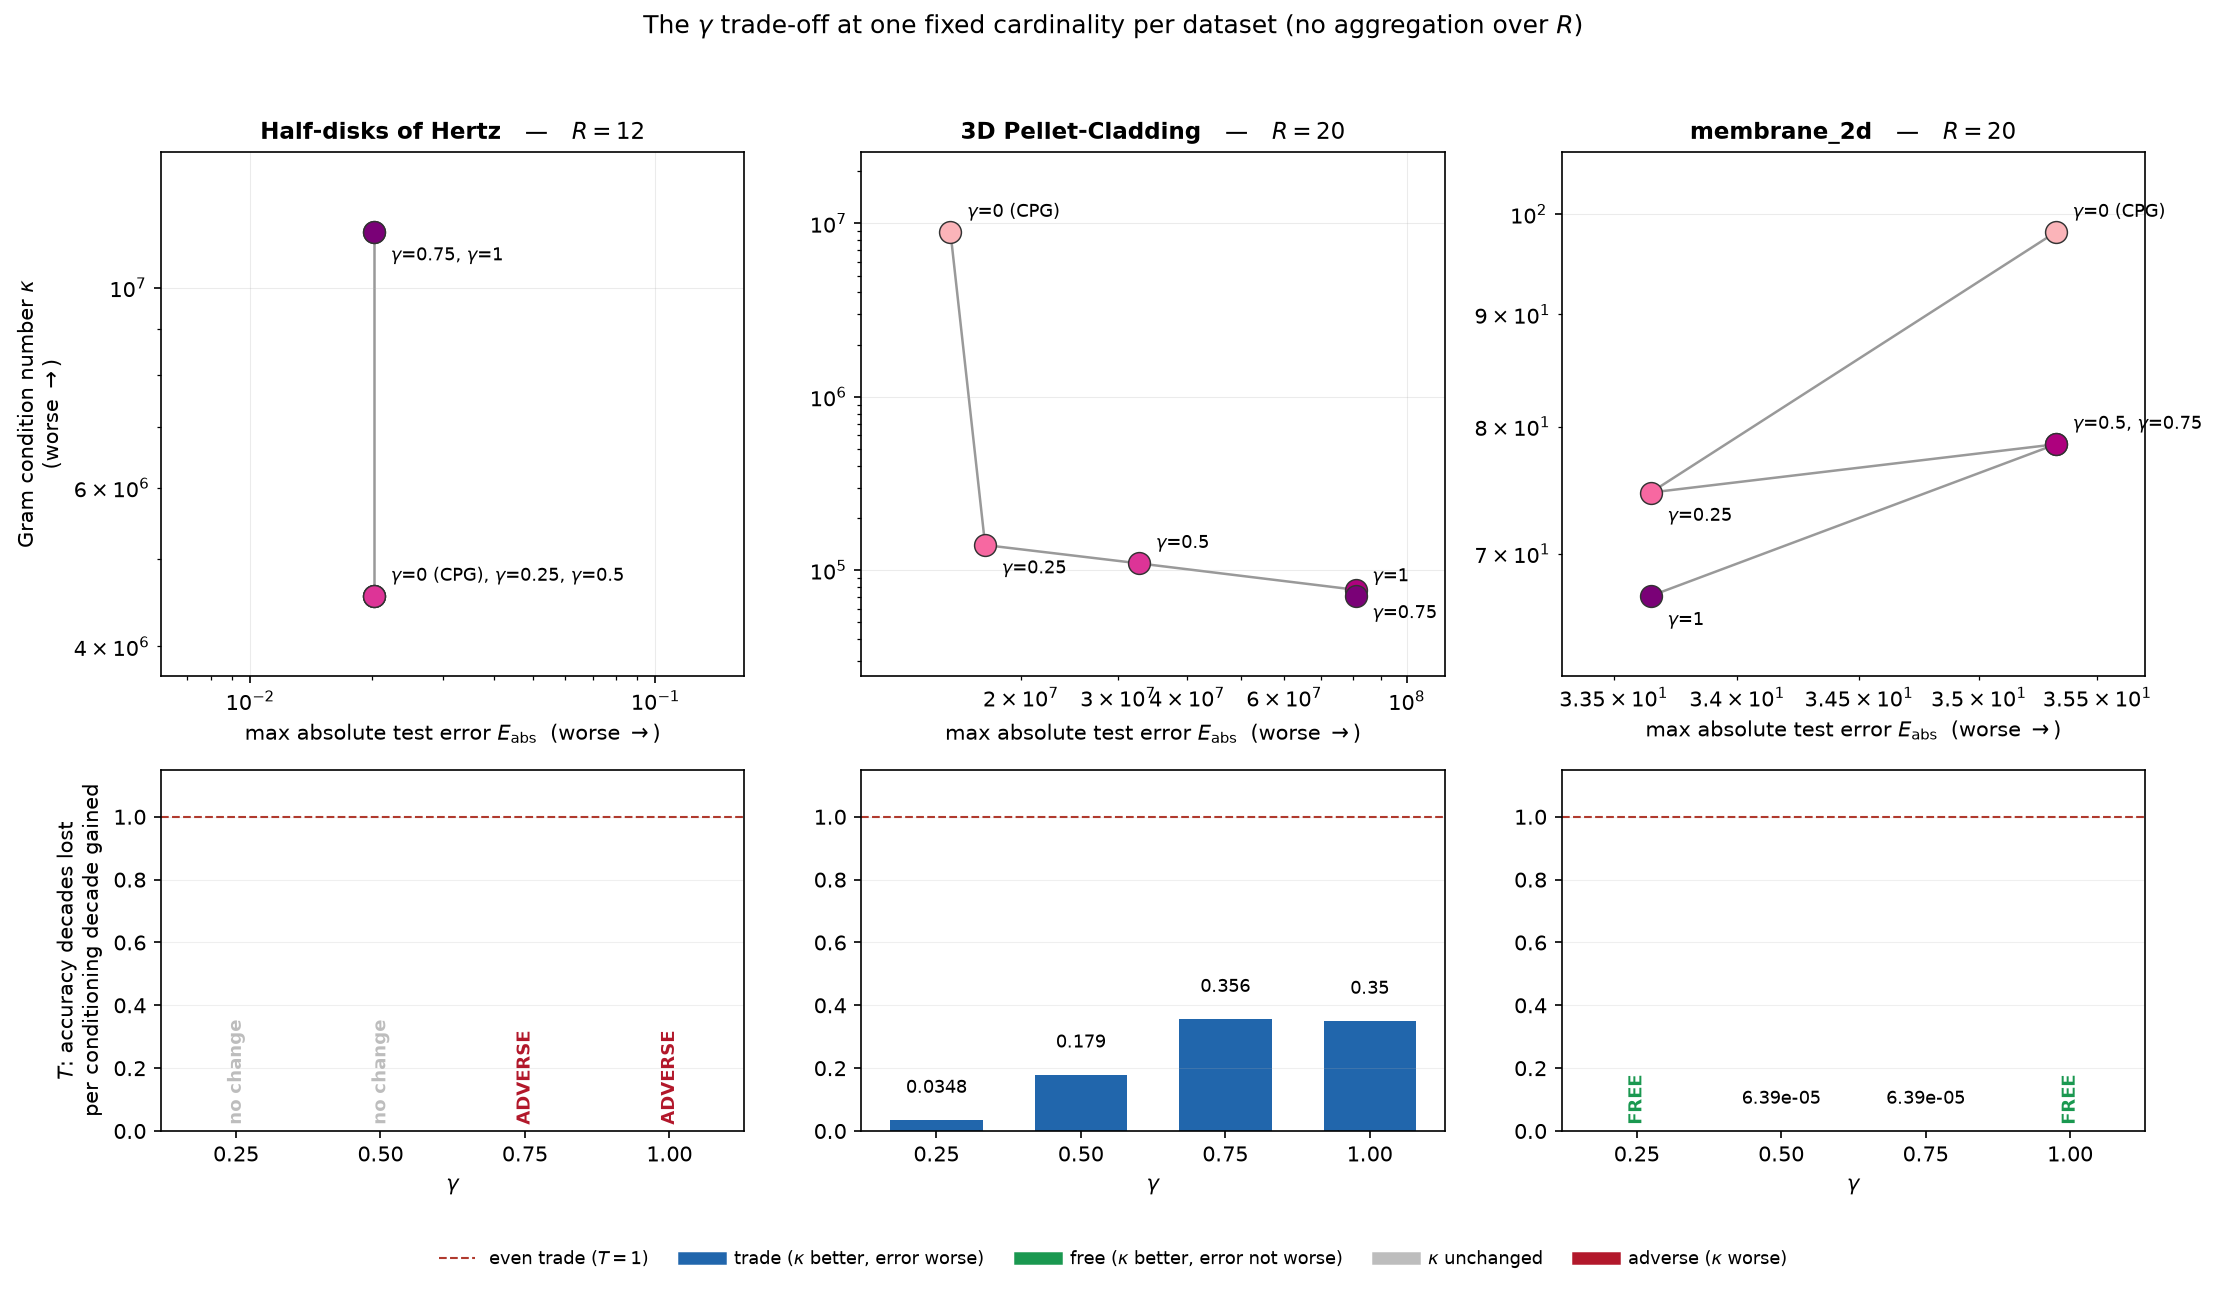
\includegraphics[width=\textwidth]{gamma_fixed_R.png}
\caption{Top: $\kappa$ against absolute test error, one point per $\gamma$, at the fixed
$R$ named in each title. Coincident members share one label. Bottom: the exchange rate
\eqref{eq:exchange} where it is defined, and the regime otherwise. Half-disks is the null
case: $\gamma\le0.5$ selects the same cone as CPG and $\gamma\ge0.75$ is strictly adverse.
Pellet-Cladding shows a sharp corner at $\gamma=0.25$. Membrane shows no trade at all ---
every member is free or neutral.}
\label{fig:fixedR}
\end{figure}

\begin{center}
\begin{tabular}{@{}llrrrr@{}}
\toprule
dataset ($R$) & $\gamma$ & $E_{\mathrm{abs}}$ & $E/E_{\mathrm{CPG}}$
& $\kappa_{\mathrm{CPG}}/\kappa_{\gamma}$ & $T$ \\
\midrule
Half-disks & $0$ (CPG) & $2.023\times10^{-2}$ & $1.000$ & $1.00$ & --- \\
$R=12$     & $0.25$    & $2.023\times10^{-2}$ & $1.000$ & $1.00$ & no change \\
           & $0.5$     & $2.023\times10^{-2}$ & $1.000$ & $1.00$ & no change \\
           & $0.75$    & $2.023\times10^{-2}$ & $1.000$ & $0.40$ & adverse \\
           & $1$       & $2.023\times10^{-2}$ & $1.000$ & $0.40$ & adverse \\
\addlinespace
Pellet-    & $0$ (CPG) & $1.490\times10^{7}$ & $1.000$ & $1.0$   & --- \\
Cladding   & $0.25$    & $1.722\times10^{7}$ & $1.156$ & $63.8$  & $\mathbf{0.035}$ \\
$R=20$     & $0.5$     & $3.276\times10^{7}$ & $2.198$ & $81.4$  & $0.179$ \\
           & $0.75$    & $8.083\times10^{7}$ & $5.424$ & $115.6$ & $0.356$ \\
           & $1$       & $8.083\times10^{7}$ & $5.424$ & $125.4$ & $0.350$ \\
\addlinespace
membrane   & $0$ (CPG) & $35.32$ & $1.000$ & $1.00$ & --- \\
$R=20$     & $0.25$    & $33.65$ & $0.953$ & $1.32$ & free \\
           & $0.5$     & $35.33$ & $1.000$ & $1.25$ & free \\
           & $0.75$    & $35.33$ & $1.000$ & $1.25$ & free \\
           & $1$       & $33.65$ & $0.953$ & $1.47$ & free \\
\bottomrule
\end{tabular}
\end{center}

\begin{figure}[htbp]
\centering
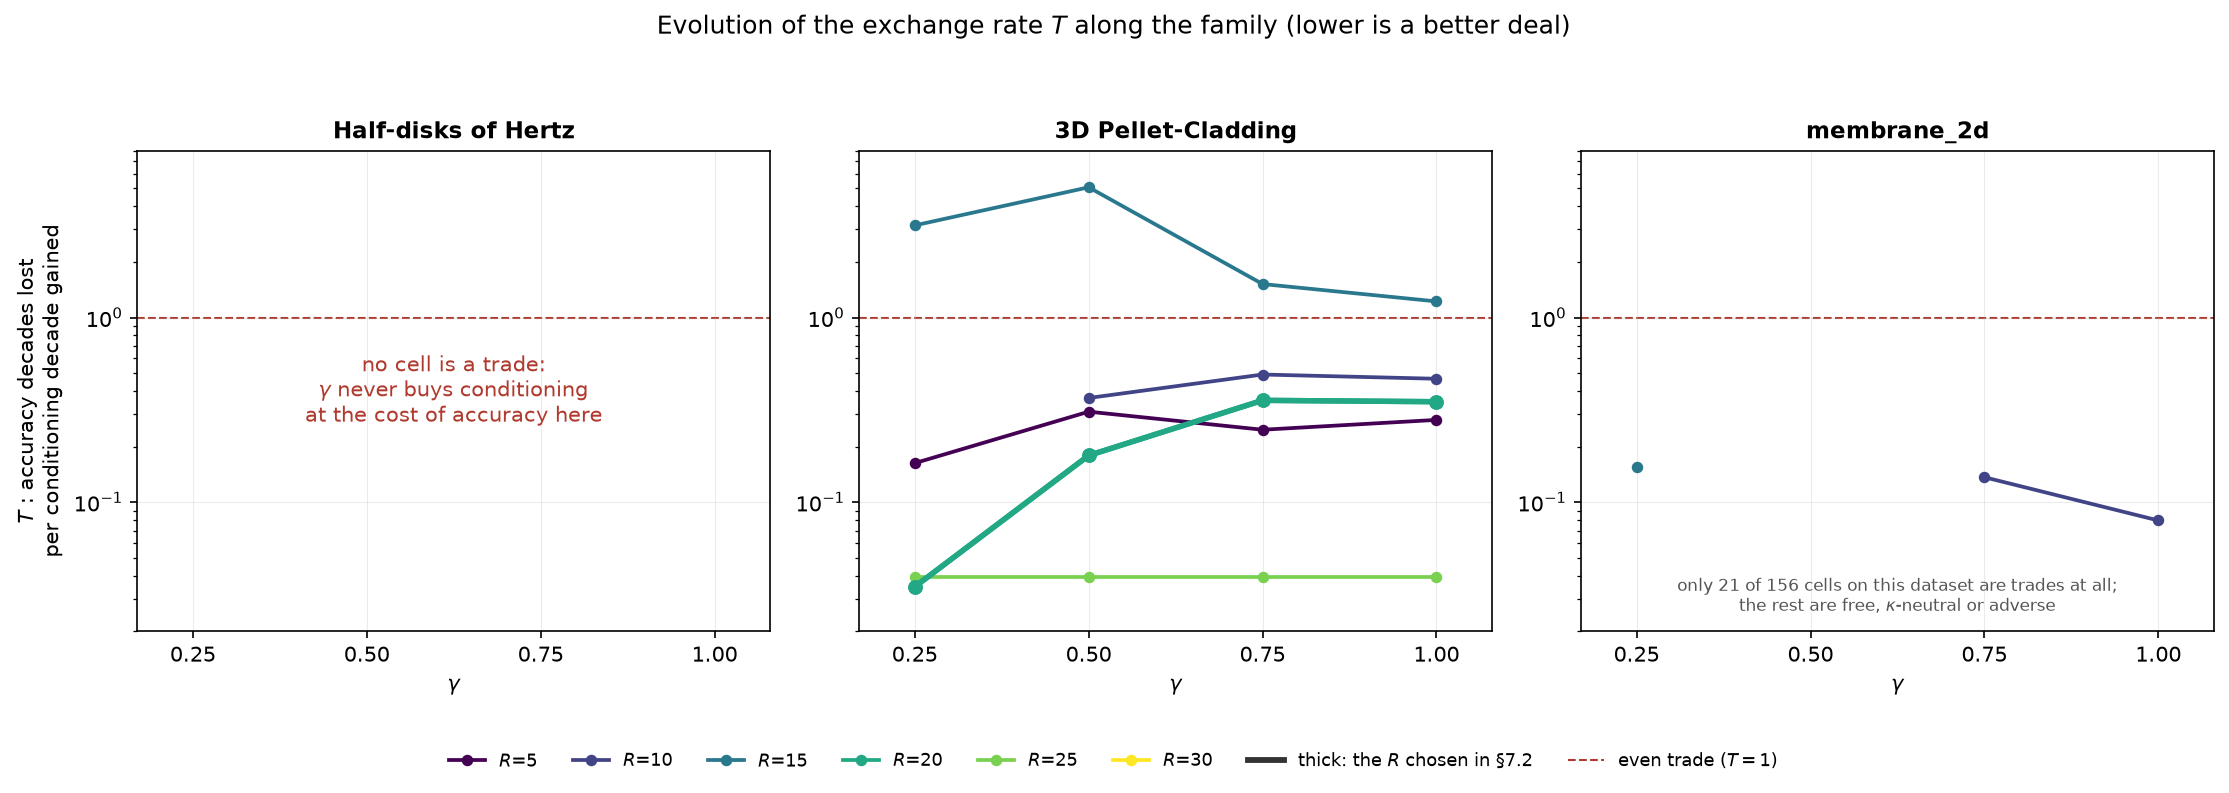
\includegraphics[width=\textwidth]{gamma_T.png}
\caption{The exchange rate \eqref{eq:exchange} against $\gamma$, one curve per
cardinality; the curve at the $R$ used in \S\ref{sec:fixedR} is drawn thick. $\gamma=0$
is absent by construction --- it is CPG against itself, so both logarithms vanish --- and
a point is plotted only where $T$ is a meaningful number, so gaps are cells that were
free, $\kappa$-neutral or adverse rather than missing runs. Half-disks has no trade at any
cardinality below its rank cliff. On Pellet-Cladding the $R=15$ curve sits \emph{above}
the even-trade line for every $\gamma$ while $R=25$ sits an order of magnitude below it,
so the same knob is poor value at one cardinality and excellent at another. Membrane has
so few trades that three points are all the family produces at these $R$.}
\label{fig:T}
\end{figure}

\noindent \textbf{Half-disks: $\gamma$ is inert, then harmful.} At $R=12$ all five members
return the identical error, $\gamma\le0.5$ returns the identical $\kappa$, and
$\gamma\ge0.75$ returns a $\kappa$ $2.5\times$ \emph{worse} for no accuracy in return.
There is nothing to trade and no reason to leave $\gamma=0$.

\noindent \textbf{Pellet-Cladding: the corner is at $\gamma=0.25$, sharply.} That member
buys $63.8\times$ the conditioning for a $1.16\times$ error, an exchange rate of
$T=0.035$ --- one decade of conditioning for three and a half percent of a decade of
accuracy. Everything past it is a much worse deal: $\gamma=0.5$ roughly doubles the
error for a further $1.3\times$ conditioning, and $\gamma=0.75$ costs $5.4\times$ the
error --- the full $\sigma^{\gamma}$ penalty --- for $115.6\times$, only $1.8\times$ more
conditioning than $\gamma=0.25$ already had. The rate degrades monotonically, $0.035 \to
0.179 \to 0.356$, so the first quarter of the $\gamma$ range contains nearly all of the
value. $\gamma=1$ is again dominated: it is indistinguishable from $\gamma=0.75$ in error
while its extra conditioning is marginal.

\noindent \textbf{Membrane: no trade exists.} Every nonzero $\gamma$ improves $\kappa$
without costing accuracy --- $\gamma=0.25$ and $\gamma=1$ are $4.7\%$ \emph{more} accurate
than CPG as well as better conditioned --- so $T$ is undefined for all of them and the
correct reading is that $\gamma$ is free here, not that it is cheap. The gains are small
in absolute terms ($1.5\times$ at most), because this dataset is well conditioned to begin
with.

\paragraph{What the rest of the sweep adds.} The three readings above are taken at one
$R$. Evaluating \eqref{eq:exchange} at every cardinality audits them, and qualifies one.
Fig.~\ref{fig:T} plots the $\gamma$-dependence at representative cardinalities; the counts
below are over the whole sweep.

\begin{itemize}
\item \textbf{Pellet-Cladding has an expensive band immediately before the cheap one.}
The only cells in the entire sweep with $T>1$ --- a worse-than-even trade --- are 19
cells confined to $R=14$--$19$, peaking at $T=5.07$ ($R=15$, $\gamma=0.5$); the $R=15$
curve in Fig.~\ref{fig:T} lies wholly above the even-trade line. At those
cardinalities CPG's $\kappa$ has not yet degraded while the family's error penalty is
already fully paid, so the exchange is bad; from $R=20$ it inverts. The knob is therefore
not merely less useful below $R=20$, it is actively poor value between $R=14$ and $R=19$,
which no summary over $R$ and no single-$R$ reading would show.
\item \textbf{The membrane recommendation is confined to $R\lesssim22$.} At $\gamma=1$ the
cells are free or trading for $R\le22$, but \emph{adverse} at 14 of the 17 cardinalities
$R\ge24$. The choice of $\gamma=1$ there is correct at $R=20$ and reverses beyond it. This
is the clearest instance of why one $R$ is a real restriction, and it is the reason
Caveat~\ref{cav:oneR} is worded as it is.
\item \textbf{Half-disks has no trade anywhere it is interpretable.} Below the rank
cliff only 4 of 60 cells are anything other than ``$\kappa$ unchanged'', and all four are
\emph{adverse} ($R=12$ and $R=14$, $\gamma\ge0.75$). Every cell in which $\gamma$ appears
to gain something lies past $R=17$, where $\kappa$ is round-off. The null result is not an
artefact of the cardinality chosen for it, which is why the left panel of
Fig.~\ref{fig:T} is empty.
\end{itemize}

\subsection{Error and conditioning as direct functions of $\gamma$}\label{sec:gammadirect}

Fig.~\ref{fig:fixedR} plots the two quantities against \emph{each other} at one fixed
cardinality. Fig.~\ref{fig:errkappa} plots them against
$\gamma$ itself, one curve per cardinality, with no aggregation --- which is what makes
the $R$-dependence visible rather than averaged away. Absolute error is recovered exactly
from the recorded relative one: the precision metric divides by a single shared
denominator, $\text{\texttt{scale}}=\max_q\|\theta_q\|$ over the training set
(\S\ref{sec:protocol}), so $E_{\mathrm{abs}}=\text{\texttt{test\_max\_rel\_err}}\times
\text{\texttt{scale}}$.

\begin{figure}[htbp]
\centering
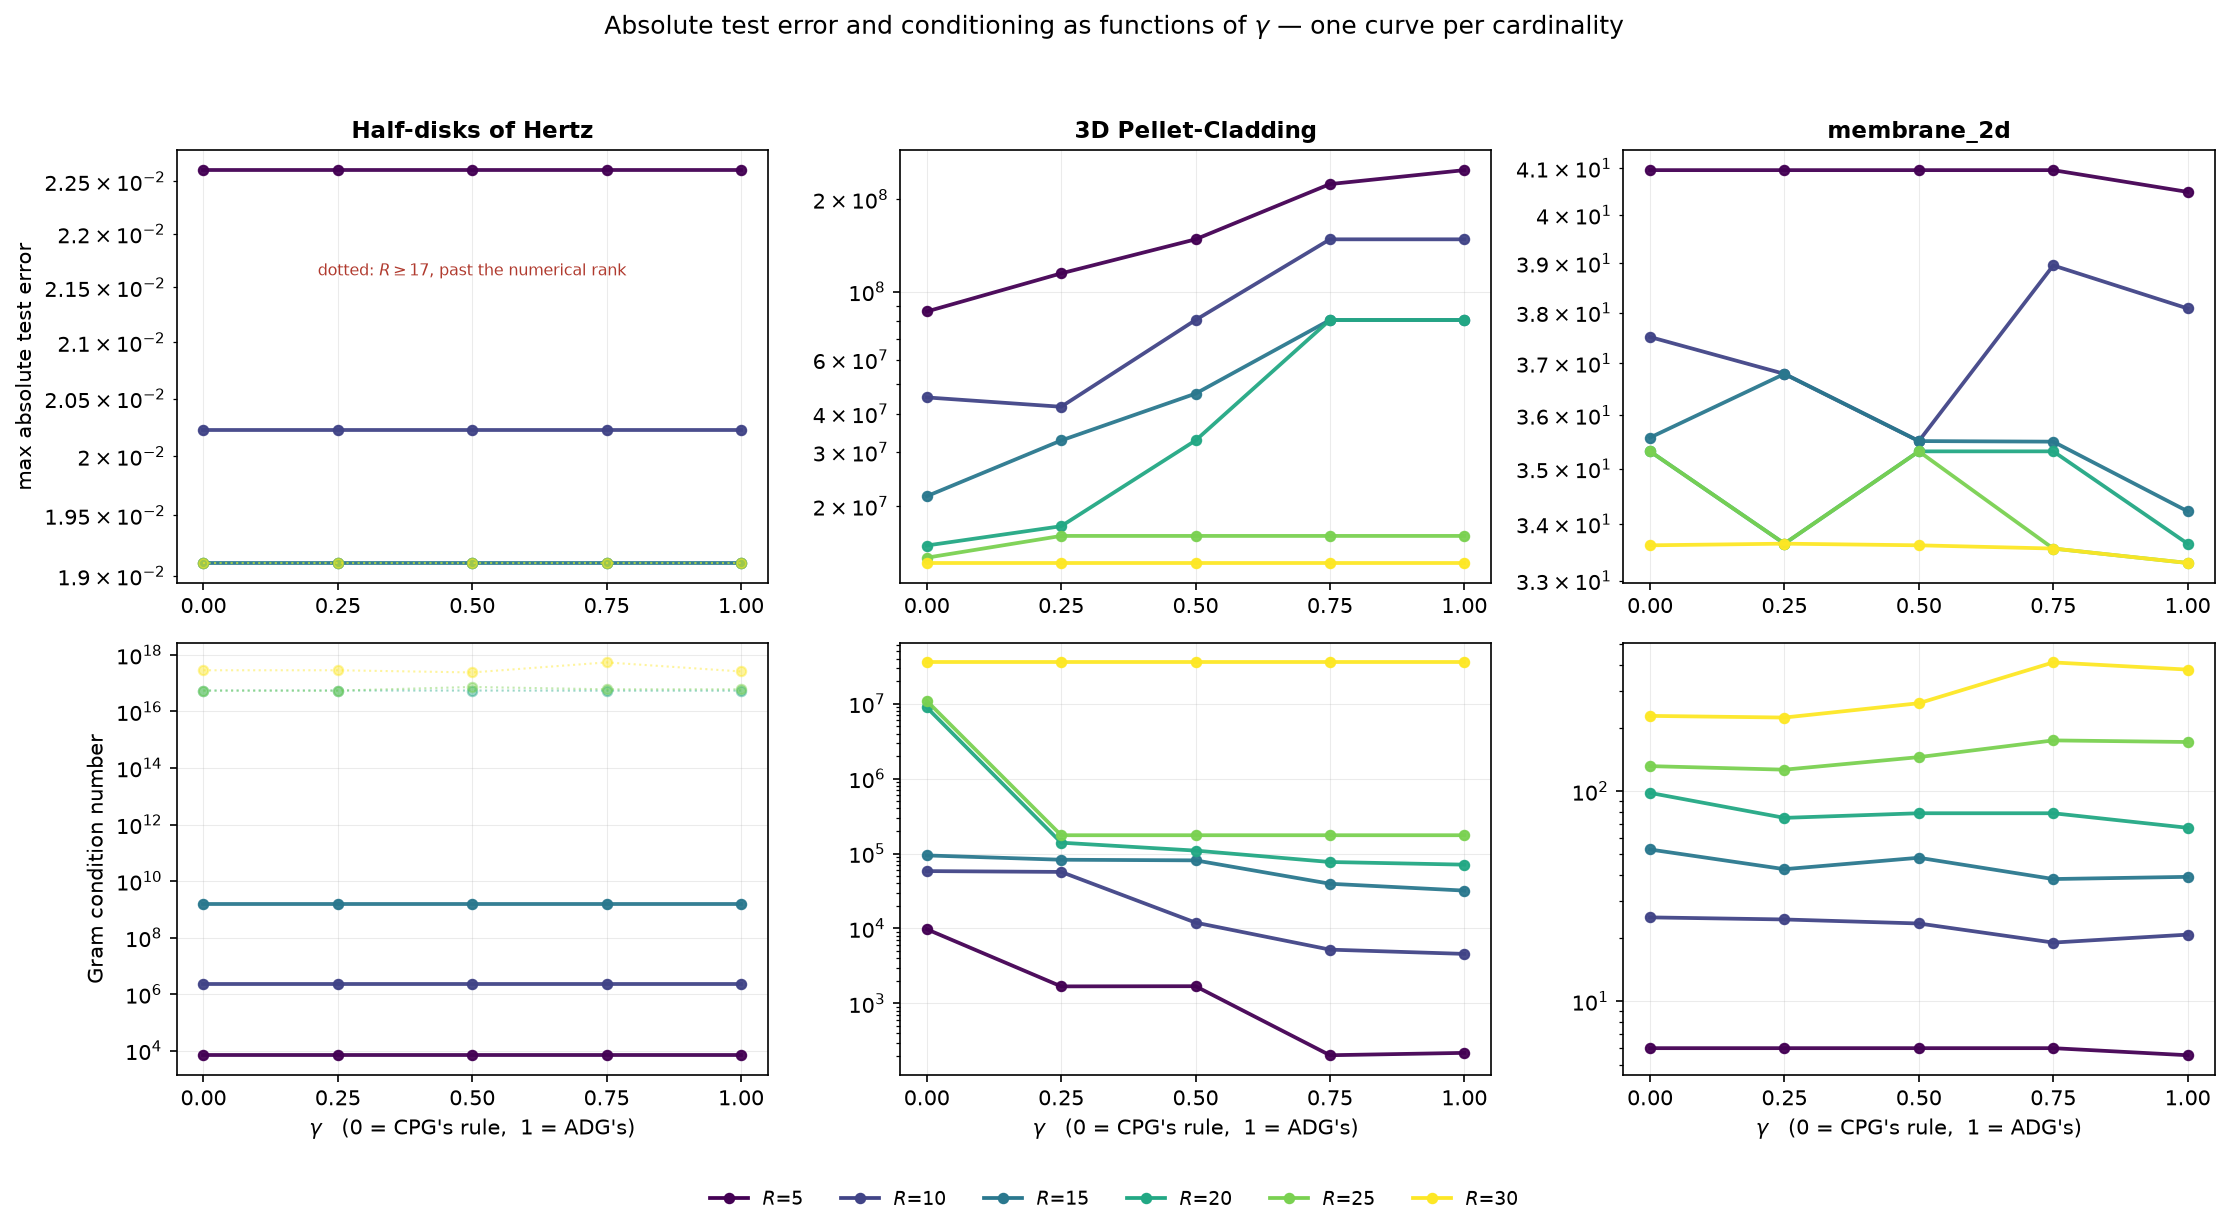
\includegraphics[width=\textwidth]{gamma_error_kappa.png}
\caption{Maximum absolute test error (top) and Gram condition number (bottom) against
$\gamma$, one curve per cardinality, for each dataset. Half-disks (left) is flat in
$\gamma$ in both rows --- the null result of \S\ref{sec:gamma}, here with no aggregation
to hide behind; the three coincident lower curves are $R\ge17$, past the numerical rank,
and are drawn dotted because their $\kappa$ is round-off. Pellet-Cladding (centre) is the
responsive case, and the two rows lean in opposite directions, which is the trade-off
stated as a picture: error rises with $\gamma$ at every $R$, $\kappa$ falls with $\gamma$
at every $R$. Note that both effects are strongest at small $R$ and vanish by $R=30$,
where all five members coincide. Membrane (right) moves by a few percent with no
consistent direction.}
\label{fig:errkappa}
\end{figure}

\noindent Two features are worth reading off the centre column directly. First, the
$\kappa$ curves are steepest between $\gamma=0$ and $\gamma=0.25$ --- at $R=20$ and
$R=25$ almost the entire drop, from $\approx10^{7}$ to $\approx2\times10^{5}$, has already
happened by $\gamma=0.25$, and the remaining three quarters of the range buy little. The
error curves over that same first step are nearly flat at those $R$. This is the same
corner \S\ref{sec:fixedR} locates at $R=20$, here visible across every $R$ at once. Second, the curves flatten from
the right as $R$ grows: at $R=25$ the error is constant for $\gamma\ge0.25$ and at $R=30$
it is constant throughout, because by then every member has selected an equivalent cone.
The knob has an operating range in $R$, and outside it there is nothing to tune.

\subsection{Which $\gamma$ to use}

Read at the fixed cardinalities of \S\ref{sec:fixedR}, with no aggregation:

\begin{itemize}
\item \textbf{Half-disks: $\gamma=0$, i.e. leave CPG alone.} The weight is inert for
$\gamma\le0.5$ and strictly harmful beyond, and the region above the rank cliff where the
family appears to separate is not interpretable.
\item \textbf{Pellet-Cladding: $\gamma=0.25$.} It captures $63.8$ of the $125.4$ available
conditioning gain for $1.16\times$ the error, where the members that capture the rest cost
$5.4\times$. This is the value the $\sigma^{\gamma}$ bound predicts should work
($\sigma=186.85$, so $\sigma^{0.25}=3.7$ bounds the loss, and the realized $1.16$ is well
inside it), and it is inside the $\gamma\approx0.2$--$0.4$ window that the norm spread
suggests a priori.
\item \textbf{Membrane: $\gamma=1$, but only for $R\lesssim22$.} At $R=20$ it has the
best conditioning of the family ($1.47\times$) and $4.7\%$ better error than CPG --- free
rather than a trade. The qualification is not cosmetic: past $R\approx24$ that member
turns adverse at 14 of the 17 cardinalities $R\ge24$, so at larger $R$ the
recommendation here is $\gamma=0$. The absolute stakes are low either way.
\end{itemize}

\begin{figure}[htbp]
\centering
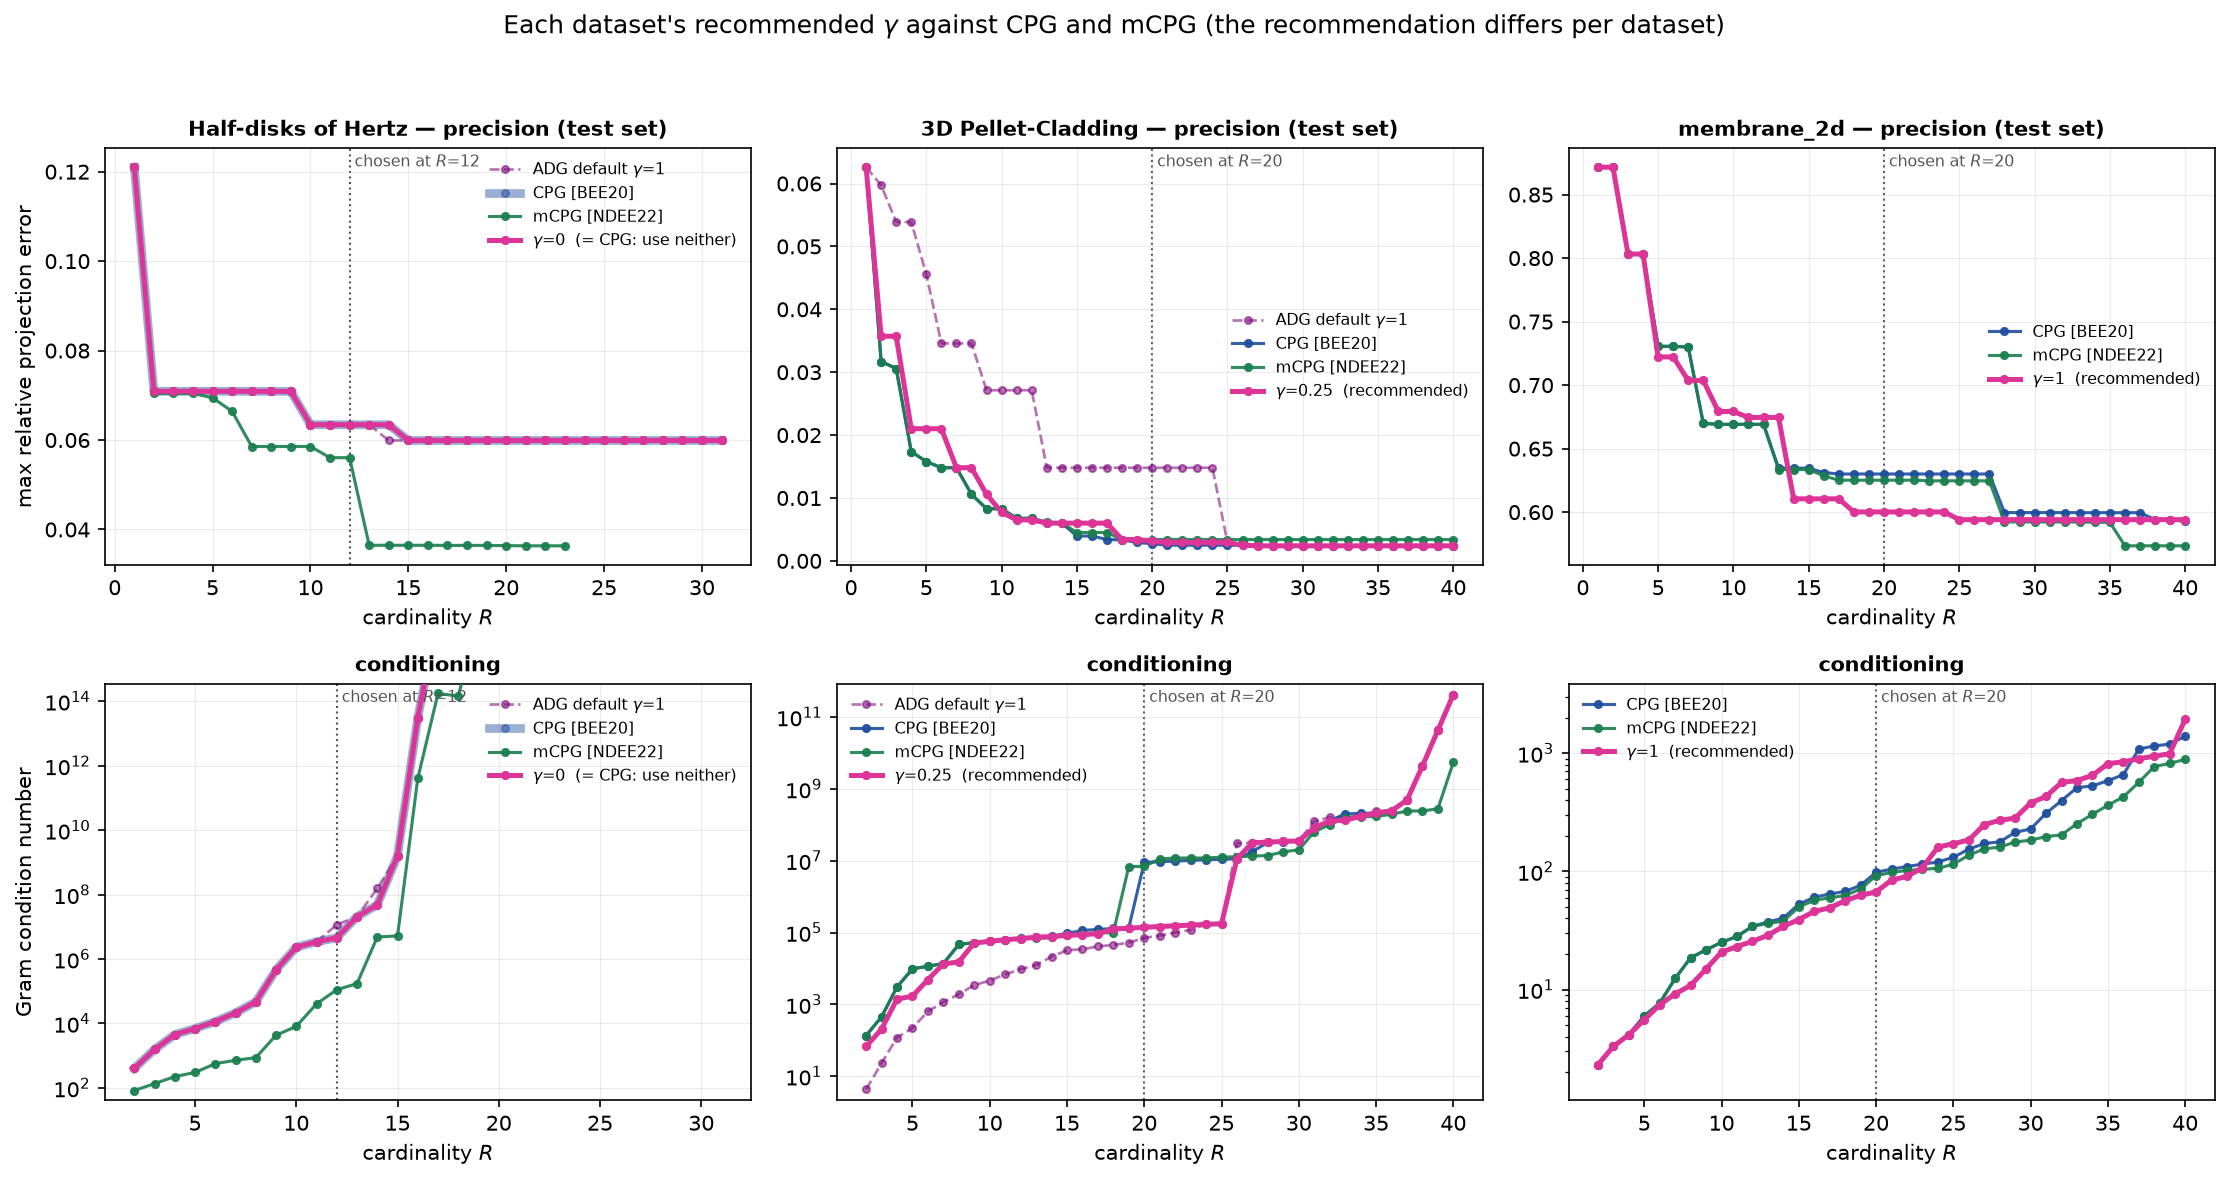
\includegraphics[width=\textwidth]{gamma_recommended.png}
\caption{Each dataset's own recommended $\gamma$ against CPG and mCPG across the whole
sweep, with the cardinality at which the recommendation was made marked. The
recommendation differs per dataset, so this is not the fixed pair drawn in the
per-dataset comparison figures. ADG's default $\gamma=1$ is shown faint and dashed
wherever it is \emph{not} the recommendation, which is what makes the cost of taking the
default visible: on Pellet-Cladding it sits far above the recommended $\gamma=0.25$ in
error for the whole range $R\lesssim25$. On Half-disks the recommendation is CPG's own
rule, so the two coincide exactly and CPG is drawn as a wide pale band beneath it; that
coincidence is the finding there, not a plotting artefact.}
\label{fig:reco}
\end{figure}

\noindent Fig.~\ref{fig:reco} shows the three recommendations against the baselines over
the full sweep, which is the check that the fixed-$R$ choice of \S\ref{sec:fixedR} is not
an artefact of that $R$: the recommended curve is at or below the $\gamma=1$ default in
error everywhere on Pellet-Cladding, not only at $R=20$.

\noindent The general statement is narrower than the family's motivation suggests. $\gamma$
is a free knob, it is well defined, and its endpoints reproduce two existing methods
exactly --- but on one of three datasets it is inert or harmful, on another it is free and
immaterial, and only on the third does the choice carry real consequences. What predicts
which case obtains is $\sigma$, computable from the snapshots before any method runs; this
is the same shape of conclusion as \S\ref{sec:cliff}, where the numerical rank predicted
the usable range.

\section{Caveats}

\begin{enumerate}
\item \textbf{No dataset currently drives a reduced solve.} The two 1-D obstacle toys were
the only sources shipping $A$, $B(\mu)$, $f$ and $g$; with them removed, the inf-sup
family and the solved-error metric report nothing on the three retained datasets. Both
remain implemented and generic, and their tests build such a problem themselves.
\item \textbf{The orthant's cost is mCPG's ordering run,} not the cone assembly, which is
free. Tracking mCPG is what buys the comparability; the price is that the cost column
measures the tracking.
\item \textbf{Extent above 1 is not an error.} It means the cone is wider than $\Kfull$,
which requires leaving it. mCPG and the orthant both do.
\item \textbf{The full-cone reference in the solved-error table is not a lower bound.} The
reduced solve minimizes over the cone rather than projecting onto it, so a smaller cone can
land closer.
\item \textbf{Half-disks results are meaningless past $R\approx15$}, and this is a
statement about the data rather than the methods: the snapshot spectrum has numerical
rank 17 of 31, so beyond that every generator is a numerically dependent combination of
those already held (\S\ref{sec:cond}). The usable range is predictable from the spectrum
before any method is run.
\item \textbf{Membrane errors are large in absolute terms} ($\approx0.6$) for every
method: 125 snapshots on 497 dual dofs with a moving contact patch is simply not
compressible to $R\le40$. Comparisons there remain valid; the absolute level is a property
of the dataset.
\item \textbf{Comparisons are matched-cardinality, not aggregated.} Every ranking in
\S\ref{sec:results}--\S\ref{sec:cond} is read at one or a few fixed $R$ from the same
sweep the figures use. A median over $R$ was tried first and discarded: it can and did
reverse rankings a matched-$R$ reading shows plainly, most visibly for NMF's apparent
Half-disks advantage (\S\ref{sec:precost}), which turned out to be confined to
cardinalities past the training set's numerical rank rather than a general property of
the method.
\item \textbf{The $\gamma$ recommendation is limited by the grid.} $\gamma=0.25$ is
the smallest nonzero value swept, and on Pellet-Cladding below $R=21$ it is the only
member that keeps error near CPG's --- so it may be at the edge of the useful range rather
than at its optimum. Whether $\gamma\in(0,0.25)$ retains the conditioning gain at a lower
error cost is not measured here.
\item\label{cav:oneR} \textbf{The $\gamma$ comparison rests on one cardinality per
dataset} ($R=12$, $20$, $20$; \S\ref{sec:fixedR}). The rule fixing them --- the numerical
rank cliff, and the smallest $R$ at which CPG is within $20\%$ of its own error floor ---
involves only CPG and the snapshot spectrum, not the $\gamma$ results, but it is a single
$R$ nonetheless, and one recommendation is known to be local to it: $\gamma=1$ on membrane
is free at $R=20$ and adverse at almost every $R\ge24$ (\S\ref{sec:fixedR}).
An earlier version of this section aggregated over the whole sweep instead and reached a
different conclusion on Pellet-Cladding ($\gamma=0.75$ rather than $\gamma=0.25$), because
every member converges in error by $R\approx25$ and a median is dominated by that tail.
Fig.~\ref{fig:T} and \S\ref{sec:gammadirect} give the exchange rate and the underlying
quantities across a range of $R$ so both the choice and its locality can be checked.
\end{enumerate}

\section*{Reproduction}
\begin{verbatim}
# --datasets defaults to all three; listed here to make the scope explicit.
python -m bench run --datasets fem_lambda physics membrane_2d \
       --subsample 200 --out results
python -m bench run --datasets fem_lambda physics membrane_2d --deltas \
       --cardinalities $(seq 1 40) --no-infsup --no-determinism \
       --subsample 200 --out results/sweep_dense
python -m bench report   --results results --out results/report.txt
python -m bench figures  --results results/sweep_dense --out results/figures --separate
python -m bench decrement --cardinality-results results/sweep_dense \
       --tolerance-results results --out results/figures
python -m bench reconstruct --R 8 --separate --out results/figures

# The gamma family (Sec. 8). Same runner, widened method set.
python -m bench run --datasets fem_lambda physics membrane_2d \\
       --methods adg_g0 adg_g25 adg_g50 adg_g75 adg_g100 cpg_bee20 mcpg_ndee22 nmf_s0 \\
       --cardinalities $(seq 1 40) --no-infsup --no-determinism \\
       --subsample 200 --out results/gamma_study
\end{verbatim}
\noindent Main grid 174/210 cells in 919\,s; dense sweep 817/840 cells in 1848\,s;
165 tests passing. The $\gamma$ grid is 960 cells.


\appendix
\section{Derivation of the reduced dual problem (Eq.~9)}\label{app:dual}

\subsection*{Step 0 --- the HF problem is a constrained minimization}
System~\eqref{eq:hf} is the KKT system of
\begin{equation}
\min_{u}\;\tfrac12 u^{\!\top}\!Au - f^{\!\top}u
\quad\text{subject to}\quad Bu\le g ,
\label{eq:primalHF}
\end{equation}
with $\lambda\ge0$ the multiplier of the inequality. $A$ is symmetric positive definite
(a stiffness matrix), which is what makes every elimination below legitimate.

\subsection*{Step 1 --- substitute the reduced ansatz}
Take $u\approx Va$ with $a\in\R^{N}$ \emph{free in sign}, and $\lambda\approx\Xi\alpha$
with $\alpha\ge0$. Testing the equilibrium equation against $V$ and the constraint against
$\Xi$ gives the reduced KKT system
\begin{equation}
\hat A a + \hat B^{\!\top}\alpha = \hat f,
\qquad \hat B a \le \hat g,
\qquad \alpha\ge0,
\label{eq:redKKT}
\end{equation}
with $\hat A=V^{\!\top}\!AV$, $\hat B=\Xi^{\!\top}\!B(\mu)V$, $\hat f=V^{\!\top}\!f$,
$\hat g=\Xi^{\!\top}g$. Equivalently: minimize $\tfrac12a^{\!\top}\hat Aa-\hat f^{\!\top}a$
subject to $\hat Ba\le\hat g$.

\subsection*{Step 2 --- eliminate $a$}
This is the step Eq.~(9) compresses. The Lagrangian of the reduced problem is
\begin{equation}
L(a,\alpha)=\tfrac12a^{\!\top}\hat Aa-\hat f^{\!\top}a+\alpha^{\!\top}(\hat Ba-\hat g).
\end{equation}
$L$ is strictly convex in $a$, so the inner minimum is attained where
$\partial_a L=\hat Aa-\hat f+\hat B^{\!\top}\alpha=0$, i.e.
\begin{equation}
a^{*}(\alpha)=\hat A^{-1}\bigl(\hat f-\hat B^{\!\top}\alpha\bigr).
\label{eq:astar}
\end{equation}
Write $s=\hat f-\hat B^{\!\top}\alpha$, so $a^{*}=\hat A^{-1}s$. Substituting,
\begin{align}
L(a^{*},\alpha)
&=\tfrac12 s^{\!\top}\hat A^{-1}s-\hat f^{\!\top}\hat A^{-1}s+(\hat B^{\!\top}\alpha)^{\!\top}\hat A^{-1}s-\alpha^{\!\top}\hat g \nonumber\\
&=\tfrac12 s^{\!\top}\hat A^{-1}s-\underbrace{(\hat f-\hat B^{\!\top}\alpha)^{\!\top}}_{=\;s^{\top}}\hat A^{-1}s-\alpha^{\!\top}\hat g
\;=\;-\tfrac12 s^{\!\top}\hat A^{-1}s-\alpha^{\!\top}\hat g .
\end{align}
Expanding $s^{\!\top}\hat A^{-1}s
=\hat f^{\!\top}\hat A^{-1}\hat f-2\alpha^{\!\top}\hat B\hat A^{-1}\hat f+\alpha^{\!\top}\hat B\hat A^{-1}\hat B^{\!\top}\alpha$
and \emph{maximizing} the dual (equivalently minimizing its negative), the constant
$\tfrac12\hat f^{\!\top}\hat A^{-1}\hat f$ drops and what remains is exactly Eq.~(9):
\begin{equation}
\boxed{\;\min_{\alpha\ge0}\;\tfrac12\,\alpha^{\!\top}Q\,\alpha-\alpha^{\!\top}c,
\qquad Q=\hat B\hat A^{-1}\hat B^{\!\top},
\qquad c=\hat B\hat A^{-1}\hat f-\hat g. \;}
\label{eq:dualQP}
\end{equation}
The displacement is then recovered from~\eqref{eq:astar}, and
$\hat\lambda=\Xi\alpha$.

\subsection*{Step 3 --- what $Q$ and $c$ mean}
Neither is an arbitrary algebraic object.
\begin{itemize}
\item $Q=\hat B\hat A^{-1}\hat B^{\!\top}$ is the \textbf{Schur complement}, i.e. the
compliance of the structure \emph{seen from the contact interface}. Entry $Q_{ij}$ is the
interface displacement in generator direction $i$ produced by a unit contact force in
direction $j$. It is symmetric positive \emph{semi}-definite.
\item $c=\hat B\hat A^{-1}\hat f-\hat g$ is the \textbf{penetration of the contact-free
solution}: $\hat A^{-1}\hat f$ is the displacement with contact ignored, $\hat B$ reads it
at the interface, and $\hat g$ is the gap. Positive entries are the penetration that
contact forces must remove.
\end{itemize}
So Eq.~\eqref{eq:dualQP} reads: \emph{choose non-negative contact-force coefficients that
undo the penetration $c$, weighted by the interface compliance $Q$.}

\subsection*{Step 4 --- in what sense it \emph{is} a projection}
The objection ``this minimizes an energy rather than projecting'' is half right. Completing
the square in the $\hat A^{-1}$ inner product $\langle x,y\rangle_{\hat A^{-1}}=x^{\!\top}\hat A^{-1}y$,
\begin{equation}
\tfrac12\alpha^{\!\top}Q\alpha-\alpha^{\!\top}c
\;=\;\tfrac12\bigl\|\hat B^{\!\top}\alpha-\hat f\bigr\|^{2}_{\hat A^{-1}}
\;+\;\alpha^{\!\top}\hat g
\;-\;\tfrac12\bigl\|\hat f\bigr\|^{2}_{\hat A^{-1}} ,
\label{eq:proj}
\end{equation}
verified numerically to $2.8\times10^{-14}$ over random $\alpha\ge0$. So the reduced solve
\emph{is} a projection --- of the load $\hat f$ onto the cone of attainable reactions
$\{\hat B^{\!\top}\alpha:\alpha\ge0\}$, in the \textbf{energy (compliance) metric}
$\hat A^{-1}$, shifted by the linear gap term $\alpha^{\!\top}\hat g$. When $\hat g=0$ it
is exactly that projection.

This is precisely why solved error and projection error are different functionals of the
same cone, as \S3.6 claims. The metric $\Pi_K$ used everywhere else in this benchmark is
the \emph{Euclidean} projection of the \emph{true multiplier} onto $W_R^+$. The solve
performs an $\hat A^{-1}$-weighted projection of the \emph{load}, offset by the gap. Two
different objects, two different inner products: a cone can be good for one and poor for
the other.

\subsection*{Step 5 --- a caution about solving \eqref{eq:dualQP}}
$Q$ is a Schur complement, so its rank is limited by the interface rather than by $R$:
with more cone generators than the contact set can distinguish it is \emph{singular}. On
the synthetic obstacle problem used to test this metric, $Q$ is rank-deficient in $60\%$ of
cells, one at rank $4$ of $6$ with $\kappa(Q)=3.7\times10^{16}$.

That defeats a naive bound-constrained solver. L-BFGS-B reports \texttt{status=0}
(converged) after eight iterations on such a cell while its KKT residual is still
$4\times10^{-3}$, landing on a worse objective than the true optimum in $10\%$ of cells.
Because it reports success, nothing downstream notices. Writing~\eqref{eq:dualQP} as a
bounded least-squares problem via the eigen-decomposition $Q=W\Lambda W^{\!\top}$ --- where
NNLS is an exact active-set method --- reaches a KKT residual of $1\times10^{-14}$ on the
same cell. The implementation runs both and returns the lower objective, so it can never
be worse than the reference it mirrors.

\end{document}
